\setcounter{section}{15}
\setcounter{subsection}{11}
\setcounter{subsubsection}{0}
% Copyright 2019 by Till Tantau
%
% This file may be distributed and/or modified
%
% 1. under the LaTeX Project Public License and/or
% 2. under the GNU Free Documentation License.
%
% See the file doc/generic/pgf/licenses/LICENSE for more details.

\section{Arrows\\箭头}
\label{section-tikz-arrows}

\subsection{Overview\\概述}

\tikzname\ allows you to add (multiple) arrow tips to the end of lines as in
\tikz [baseline] \draw [->>] (0,.5ex) -- (3ex,.5ex); or in \tikz [baseline]
\draw [-{Latex[]}] (0,.5ex) -- (3ex,.5ex);. It is possible to change which
arrow tips are used ``on-the-fly'', you can have several arrow tips in a row,
and you can change the appearance of each of them individually using a special
syntax. The following example is a perhaps slightly ``excessive'' demonstration
of what you can do (you need to load the |arrows.meta| library for it to work):

\tikzname\ 允许你在线段的末尾添加(多个)箭头,例如 \tikz [baseline] \draw [->>] (0,.5ex) -- (3ex,.5ex); 或者 \tikz [baseline]
\draw [-{Latex[]}] (0,.5ex) -- (3ex,.5ex);。你可以在运行时改变使用的箭头样式,可以连续使用多个箭头,还可以使用特殊语法单独改变每个箭头的外观。下面的示例可能有点过分,但演示了你可以做的事情(需要加载 |arrows.meta| 库才能正常工作):


\begin{codeexample}[preamble={\usetikzlibrary{arrows.meta,bending,positioning}}]
\tikz {
  \node [circle,draw] (A)              {A};
  \node [circle,draw] (B) [right=of A] {B};

  \draw [draw = blue, thick,
         arrows={
           Computer Modern Rightarrow [sep]
         - Latex[blue!50,length=8pt,bend,line width=0pt]
           Stealth[length=8pt,open,bend,sep]}]
    (A) edge [bend left=45] (B)
    (B) edge [in=-110, out=-70,looseness=8] (B);
}
\end{codeexample}

There are a number of predefined generic arrow tip kinds whose appearance you
can modify in many ways using various options. It is also possible to define
completely new arrow tip kinds, see Section~\ref{section-arrows}, but doing
this is somewhat harder than configuring an existing kind (it is like the
difference between using a font at different sizes or faces like italics,
compared to designing a new font yourself).

有许多预定义的通用箭头样式,你可以使用各种选项进行修改。还可以定义全新的箭头样式,详见第~\ref{section-arrows}节,但相比配置现有样式,这样做要困难一些(就像使用不同大小或格式(如斜体)的字体与设计自己的字体之间的区别一样)。

In the present section, we go over the various ways in which you can configure
which particular arrow tips are \emph{used}. The glorious details of how new
arrow tips can be defined are explained in Section~\ref{section-arrows}.

在本节中,我们将介绍配置使用特定箭头样式的各种方法。如何定义新的箭头样式的详细信息请参见第~\ref{section-arrows}节。

At the end of the present section, Section~\ref{section-arrows-meta}, you will
find a description of the different predefined arrow tips from the
|arrows.meta| library.

在本节末尾的第~\ref{section-arrows-meta}节中,你将找到来自 |arrows.meta| 库的不同预定义箭头样式的描述。

\emph{Remark:} Almost all of the features described in the following were
introduced in version 3.0 of \tikzname. For compatibility reasons, the old
arrow tips are still available. To differentiate between the old and new arrow
tips, the following rule is used: The new, more powerful arrow tips start with
an uppercase letter as in |Latex|, compared to the old arrow tip |latex|.

\emph{注意:}下面描述的几乎所有功能都是在 \tikzname 的 3.0 版本中引入的。为了保持兼容性,旧的箭头样式仍然可用。为了区分旧的和新的箭头样式,使用了以下规则:新的、功能更强大的箭头样式以大写字母开头,例如 |Latex|,而旧的箭头样式为 |latex|。

\emph{Remark:} The libraries |arrows| and |arrows.spaced| are deprecated. Use
|arrows.meta| instead/additionally, which allows you to do all that the old
libraries offered, plus much more. However, the old libraries still work and
you can even mix old and new arrow tips (only, the old arrow tips cannot be
configured in the ways described in the rest of this section; saying |scale=2|
for a |latex| arrow has no effect for instance, while for |Latex| arrows it
doubles their size as one would expect.)

\emph{注意:}库 |arrows| 和 |arrows.spaced| 已过时。请改用 |arrows.meta|,它可以实现旧库所提供的所有功能,并且还有更多功能。但是,旧的库仍然可用,甚至可以混合使用旧的和新的箭头样式(只是旧的箭头样式无法按本节其余部分所述的方式进行配置;例如对于 |latex| 箭头使用 |scale=2| 不起作用,而对于 |Latex| 箭头会将其大小加倍,正如人们所期望的那样。)


\subsection{Where and When Arrow Tips Are Placed\\箭头的位置和时间}
\label{section-arrow-tips-where}

In order to add arrow tips to the lines you draw, the following conditions must
be met:


为了在绘制的线段上添加箭头,必须满足以下条件:
%
\begin{enumerate}
    \item You have specified that arrow tips should be added to lines, using
        the |arrows| key or its short form.

        使用 |arrows| 键或其简写形式指定了要在线段上添加箭头。
    \item You set the |tips| key to some value that causes tips to be drawn
        (to be explained later).

        将 |tips| 键设置为某个值,使得箭头可以被绘制(稍后会解释)。
    \item You do not use the |clip| key (directly or indirectly) with the
        current path.

        不使用 |clip| 键(直接或间接地)与当前路径。
    \item The path actually has two ``end points'' (it is not ``closed'').

    路径实际上有两个“端点”(不是“闭合”的)。
\end{enumerate}

Let us start with an introduction to the basics of the |arrows| key:

让我们从 |arrows| 键的基础知识介绍开始:

\begin{key}{/tikz/arrows=\meta{start arrow specification}|-|\meta{end arrow specification}}
    This option sets the arrow tip(s) to be used at the start and end of lines.
    An empty value as in |->| for the start indicates that no arrow tip should
    be drawn at the start.%
    \indexoption{arrows}
    该选项设置线段的起始和结束处要使用的箭头样式。起始处为空值,如 |->|,表示起始处不绘制箭头。%

    \emph{Note: Since the arrow option is so often used, you can leave out the
    text |arrows=|.} What happens is that every (otherwise unknown) option that
    contains a |-| is interpreted as an arrow specification.

    \emph{注意:由于箭头选项经常使用,你可以省略文本 |arrows=|。}这样做的效果是,每个(否则未知的)包含 |-| 的选项都会被解释为箭头规范。%


    %
\begin{codeexample}[preamble={\usetikzlibrary{arrows.meta}}]
\begin{tikzpicture}
  \draw[->]        (0,0)   -- (1,0);
  \draw[>-Stealth] (0,0.3) -- (1,0.3);
\end{tikzpicture}
\end{codeexample}

    In the above example, the first start specification is empty and the second
    is |>|. The end specifications are |>| for the first line and |Stealth| for
    the second line. Note that it makes a difference whether |>| is used in a
    start specification or in an end specification: In an end specification it
    creates, as one would expect, a pointed tip  at the end of the line. In the
    start specification, however, it creates a ``reversed'' version if this
    arrow -- which happens to be what one would expect here.

    在上面的例子中,第一个起始规范为空,第二个为|>|。第一行的结束规范为|>|,第二行为|Stealth|。请注意,|>|在起始规范和结束规范中使用会有所不同:在结束规范中,它会在线的末尾创建一个尖端箭头,符合预期。然而,在起始规范中,它会创建一个“反转”的箭头版本 - 这正是在这里所期望的。

The above specifications are very simple and only select a single arrow tip
    without any special configuration options, resulting in the ``natural''
    versions of these arrow tips. It is also possible to ``configure'' arrow
    tips in many different ways, as explained in detail in
    Section~\ref{section-arrow-config} below by adding options in square
    brackets following the arrow tip kind:
    
    上述规范非常简单,只选择一个单独的箭头尖端,没有任何特殊配置选项,得到的是这些箭头尖端的“自然”版本。也可以通过在箭头尖端类型之后的方括号中添加选项来以多种不同的方式“配置”箭头尖端,详细说明在下文的第~\ref{section-arrow-config}~节中。
\begin{codeexample}[preamble={\usetikzlibrary{arrows.meta}}]
\begin{tikzpicture}
  \draw[-{Stealth[red]}] (0,0)   -- (1,0);
\end{tikzpicture}
\end{codeexample}

    Note that in the example I had to surround the end specification by braces.
    This is necessary so that \tikzname\ does not mistake the closing square
    bracket of the |Stealth| arrow tip's options for the end of the options of
    the |\draw| command. In general, you often need to add braces when
    specifying arrow tips except for simple case like |->| or |<<->|, which are
    pretty frequent, though. When in doubt, say
    |arrows={|\meta{start spec}|-|\meta{end spec}|}|, that will always work.

    请注意,在示例中,我不得不用大括号括起结束规范。这是必要的,以免\tikzname\ 将|Stealth|箭头尖端选项的闭合方括号误认为是|\draw|命令选项的结束。通常情况下,在指定箭头尖端时,除了像|->|或|<<->|这样的简单情况外,通常需要添加大括号,这是相当常见的情况。如果不确定,可以使用|arrows={|\meta{起始规范}|-|\meta{结束规范}|}|,这样总是有效的。

It is also possible to specify multiple (different) arrow tips in a row
    inside a specification, see Section~\ref{section-arrow-spec} below for
    details.

    还可以在规范中连续指定多个(不同的)箭头尖端,请参阅下文的第~\ref{section-arrow-spec}~节获取详细信息。


\end{key}

As was pointed out earlier, to add arrow tips to a path, the path must have
``end points'' and not be ``closed'' -- otherwise adding arrow tips makes
little sense, after all. However, a path can actually consist of several
subpath, which may be open or not and may even consist of only a single point
(a single move-to). In this case, it is not immediately obvious, where arrow
heads should be placed. The actual rules that \tikzname\ uses are governed by
the setting of the key |tips|:

正如前面提到的,要在路径中添加箭头尖端,路径必须具有“终点”,而不能是“闭合”的-否则添加箭头尖端就没有意义。然而,路径实际上可以由多个子路径组成,这些子路径可以是开放的或非开放的,甚至可以只包含一个点(单个移动到)。在这种情况下,箭头应放置在哪里并不明显。\tikzname\ 使用的实际规则由|tips|键的设置控制:

\begin{key}{/pgf/tips=\meta{value} (default true, initially on draw)}
        \keyalias{tikz}
    This key governs in what situations arrow tips are added to a path. The
    following \meta{values} are permissible:

    此键控制在何种情况下将箭头添加到路径中。可以使用以下\meta{values}:
    %
    \begin{itemize}
        \item |true| (the value used when no \meta{value} is specified)

        |true|(当未指定\meta{value}时使用的值)
        \item |proper|
        \item |on draw| (the initial value, if the key has not yet been used
            at all)

            |on draw|(如果尚未使用该键,则为初始值)
        \item |on proper draw|
        \item |never| or |false| (same effect)

        |never|或|false|(具有相同的效果)
    \end{itemize}

    Firstly, there are a whole bunch of situations where the setting of
    these (or other) options causes no arrow tips to be shown:
    
    首先,有许多情况下这些(或其他)选项的设置不会显示箭头尖端:

    \begin{itemize}
        \item If no arrow tips have been specified (for instance, by having
            said |arrows=-|), no arrow tips are drawn.

            如果未指定箭头尖端(例如,通过使用|arrows=-|),则不会绘制箭头尖端。

        \item If the |clip| option is set, no arrow tips are drawn.

        如果设置了|clip|选项,则不会绘制箭头尖端。
        \item If |tips| has been set to |never| or |false|, no arrow tips are
            drawn.
        
            如果将|tips|设置为|never|或|false|,则不会绘制箭头尖端。

            \item If |tips| has been set to |on draw| or |on proper draw|, but
            the |draw| option is not set, no arrow tips are drawn.

        如果将|tips|设置为|on draw|或|on proper draw|,但未设置|draw|选项,则不会绘制箭头尖端。

\item If the path is empty (as in |\path ;|), no arrow tips are
            drawn.

        如果路径为空(如|\path ;|),则不会绘制箭头尖端。

\item If at least one of the subpaths of a path is closed (|cycle| is
            used somewhere or something like |circle| or |rectangle|), arrow
            tips are never drawn anywhere -- even if there are open subpaths.

            如果路径的至少一个子路径是闭合的(在某处使用了|cycle|或类似的|circle|或|rectangle|),则箭头尖端永远不会绘制-即使存在开放的子路径。
    \end{itemize}

    Now, if we pass all of the above tests, we must have a closer look at the
    path. All its subpaths must now be open and there must be at least one
    subpath. We consider the last one. Arrow tips will only be added to this
    last subpath.

    现在,如果通过了上述所有测试,我们必须仔细查看路径。所有子路径现在都必须是开放的,并且必须至少有一个子路径。我们考虑最后一个子路径。箭头尖端将仅添加到最后一个子路径中。

    \begin{enumerate}
        \item If this last subpath not degenerate (all coordinates on the
            subpath are the same as in a single ``move-to'' |\path (0,0);| or
            in a ``move-to'' followed by a ``line-to'' to the same position
            as in |\path (1,2) -- (1,2)|), arrow tips are added to this last
            subpath now.

            如果最后一个子路径不退化(子路径上的所有坐标与单个“移动到”|\path (0,0);|或以“移动到”开头并以与|\path (1,2) -- (1,2)|相同位置结尾的“线到”操作中的坐标相同),则现在在该最后一个子路径上添加箭头。


        \item If the last subpath is degenerate, we add arrow tips pointing
            upward at the single coordinate mentioned in the path, but only
            for |tips| begin set to |true| or to |on draw| -- and not for
            |proper| nor for |on proper draw|. In other words, ``proper''
            suppresses arrow tips on degenerate paths.

            如果最后一个子路径是退化的,则仅在路径中提到的单个坐标处添加指向上方的箭头,但仅对于|tips|设置为|true|或|on draw|时添加,而不对于|proper|或|on proper draw|。换句话说,“proper”会禁止在退化路径上添加箭头。

    \end{enumerate}

\begin{codeexample}[]
% No path, no arrow tips:
\tikz [<->] \draw;
\end{codeexample}
\begin{codeexample}[]
% Degenerate path, draw arrow tips (but no path, it is degenerate...)
\tikz [<->] \draw (0,0);
\end{codeexample}
\begin{codeexample}[]
% Degenerate path, tips=proper suppresses arrows
\tikz [<->] \draw [tips=proper] (0,0);
\end{codeexample}
\begin{codeexample}[]
% Normal case:
\tikz [<->] \draw (0,0) -- (1,0);
\end{codeexample}
\begin{codeexample}[]
% Two subpaths, only second gets tips
\tikz [<->] \draw (0,0) -- (1,0) (2,0) -- (3,0);
\end{codeexample}
\begin{codeexample}[]
% Two subpaths, second degenerate, but still gets tips
\tikz [<->] \draw (0,0) -- (1,0) (2,0);
\end{codeexample}
\begin{codeexample}[]
% Two subpaths, second degenerate, proper suppresses them
\tikz [<->] \draw [tips=on proper draw] (0,0) -- (1,0) (2,0);
\end{codeexample}
\begin{codeexample}[]
% Two subpaths, but one is closed: No tips, even though last subpath is open
\tikz [<->] \draw (0,0) circle[radius=2pt] (2,0) -- (3,0);
\end{codeexample}
    %
\end{key}

One common pitfall when arrow tips are added to a path should be addressed
right here at the beginning: When \tikzname\ positions an arrow tip at the
start, for all its computations it only takes into account the first segment of
the subpath to which the arrow tip is added. This ``first segment'' is the
first line-to or curve-to operation (or arc or parabola or a similar operation)
of the path; but note that decorations like |snake| will add many small line
segments to paths. The important point is that if this first segment is very
small, namely smaller that the arrow tip itself, strange things may result. As
will be explained in Section~\ref{section-arrow-flex}, \tikzname\ will modify
the path by shortening the first segment and shortening a segment below its
length may result in strange effects. Similarly, for tips at the end of a
subpath, only the last segment is considered.

在添加箭头到路径时的一个常见陷阱应该在此处进行解释:当\tikzname\ 将箭头定位在起点时,对于所有计算,它仅考虑要添加箭头的子路径的第一段。这个“第一段”是路径的第一个线到或曲线到操作(或弧线或抛物线或类似的操作);但请注意,像|snake|这样的装饰会在路径中添加许多小线段。重要的是,如果这个第一段非常小,即小于箭头本身,可能会产生奇怪的结果。正如在第\ref{section-arrow-flex}节中将解释的那样,\tikzname\ 将通过缩短第一段来修改路径,并且缩短其长度下面的一段可能会产生奇怪的效果。类似地,对于子路径末尾的箭头,只考虑最后一段。

The bottom line is that wherever an arrow tip is added to a path, the line
segment where it is added should be ``long enough''.

底线是,无论在路径的哪个位置添加箭头,添加箭头的线段应该足够“长”。


\subsection{Arrow Keys: Configuring the Appearance of a Single Arrow Tip\\箭头键:配置单个箭头的外观}
\label{section-arrow-config}

For standard arrow tip kinds, like |Stealth| or |Latex| or |Bar|, you can
easily change their size, aspect ratio, color, and other parameters. This is
similar to selecting a font face from a font family: \emph{``This text''} is
not just typeset in the font ``Computer Modern'', but rather in ``Computer
Modern, italic face, 11pt size, medium weight, black color, no underline,
\dots'' Similarly, an arrow tip is not just a ``Stealth'' arrow tip, but rather
a ``Stealth arrow tip at its natural size, flexing, but not bending along the
path, miter line caps, draw and fill colors identical to the path draw color,
\dots''

对于标准箭头类型,如|Stealth|、|Latex|或|Bar|,您可以轻松更改其大小、长宽比、颜色和其他参数。这类似于从字体系列中选择字体样式:\emph{“此文本”}不仅在“Computer Modern”字体中排版,而是在“Computer Modern,斜体,11pt大小,中等粗细,黑色,无下划线,……”字体样式中排版。类似地,箭头不仅仅是一个“Stealth”箭头,而是一个“Stealth箭头,其自然大小,弯曲但不沿路径弯曲,斜面线端,绘制和填充颜色与路径绘制颜色相同,……”

Just as most programs make it easy to ``configure'' which font should be used
at a certain point in a text, \tikzname\ tries to make it easy to specify which
configuration of an arrow tip should be used. You use \emph{arrow keys}, where
a certain parameter like the |length| of an arrow is set to a given value using
the standard key--value syntax. You can provide several arrow keys following an
arrow tip kind in  an arrow tip specification as in
|Stealth[length=4pt,width=2pt]|.

就像大多数程序可以轻松“配置”在文本中的某一点使用的字体一样,\tikzname\ 试图使其易于指定应使用的箭头样式的配置方式。您可以使用\emph{箭头键},其中某个参数(如箭头的|length|)使用标准键值语法设置为给定值。您可以在箭头尖端规范中的箭头类型后面提供多个箭头键,如|Stealth[length=4pt,width=2pt]|。

While selecting a font may be easy, \emph{designing} a new font is a highly
creative and difficult process and more often than not, not all faces of a font
are available on any given system. The difficulties involved in designing a new
arrow tip are somewhat similar to designing a new letter for a font and, thus,
it may also happen that not all configuration options are actually implemented
for a given arrow tip. Naturally, for the standard arrow tips, all
configuration options are available -- but for special-purpose arrow tips it
may well happen that an arrow tip kind simply ``ignores'' some of the
configurations given by you.

% 虽然选择字体可能很容易,但\emph{设计}新字体是一个极具创造性和困难的过程,而且往往情况下,并非所有字体的所有字形都在任何给定的系统上都可用。设计新箭头的难度与设计字体的新字母有些相似,因此,对于给定的箭头,可能并非所有配置选项都实际上被实现。当然,对于标准箭头,所有配置选项都是可用的,但对于特定用途的箭头,可能会发现某种箭头类型如果最后一个子路径不是退化的(子路径上的所有坐标与单个“移动到”命令|\path (0,0);|或者以“移动到”命令后面的“线到”命令到相同位置|\path (1,2) -- (1,2)|),则现在给这个最后的子路径添加箭头。

虽然选择字体可能很容易,但是\emph{设计}一个新字体是一个非常富有创造性和困难的过程,往往并不是所有字体的所有字形都在任何给定的系统上都可用。设计新箭头的困难与设计字体的新字母相似,因此可能并非所有配置选项都实际上适用于特定的箭头类型。当然,对于标准箭头类型,所有配置选项都是可用的,但对于特殊用途的箭头类型,箭头类型可能会“忽略”您提供的某些配置。

Some of the keys explained in the following are defined in the library
|arrows.meta|, others are always available. This has to do with the question of
whether the arrow key needs to be supported directly in the \pgfname\ core or
not. In general, the following explanations assume that |arrows.meta| has been
loaded.

下面解释的一些键是在|arrows.meta|库中定义的,另一些键则始终可用。这与箭头键是否需要在\pgfname\ 核心中直接支持有关。一般来说,以下解释假设已加载了|arrows.meta|。



\subsubsection{Size\\大小}

The most important configuration parameter of an arrow tip is undoubtedly its
size. The following two keys are the main keys that are important in this
context:

箭头尖的最重要的配置参数无疑是其大小。以下两个键是在这个上下文中非常重要的主要键:

\begin{key}{/pgf/arrow keys/length=\meta{dimension}| |\opt{\meta{line width factor}}%
        | |\opt{\meta{outer factor}}}
        \label{length-arrow-key}%
    This parameter is usually the most important parameter that governs the
    size of an arrow tip: The \meta{dimension} that you provide dictates the
    distance from the ``very tip'' of the arrow to its ``back end'' along the
    line:
    
    这个参数通常是决定箭头尺寸最重要的参数:您提供的\meta{dimension}决定了箭头从箭头的“尖端”到沿着线的“背部”的距离:
\begin{codeexample}[preamble={\usetikzlibrary{arrows.meta}}]
\tikz{
  \draw [-{Stealth[length=5mm]}] (0,0) -- (2,0);
  \draw [|<->|] (1.5,.4) -- node[above=1mm] {5mm} (2,.4);
}
\end{codeexample}
\begin{codeexample}[preamble={\usetikzlibrary{arrows.meta}}]
\tikz{
  \draw [-{Latex[length=5mm]}] (0,0) -- (2,0);
  \draw [|<->|] (1.5,.4) -- node[above=1mm] {5mm} (2,.4);
}
\end{codeexample}
\begin{codeexample}[preamble={\usetikzlibrary{arrows.meta}}]
\tikz{
  \draw [-{Classical TikZ Rightarrow[length=5mm]}] (0,0) -- (2,0);
  \draw [|<->|] (1.5,.6) -- node[above=1mm] {5mm} (2,.6);
}
\end{codeexample}

    \medskip
    \noindent \textbf{The Line Width Factors.}
    Following the \meta{dimension}, you may put a space followed by a
    \meta{line width factor}, which must be a plain number (no |pt| or |cm|
    following). When you provide such a number, the size of the arrow tip is
    not just \meta{dimension}, but rather $\meta{dimension} + \meta{line width
    factor}\cdot w$ where $w$ is the width of the to-be-drawn path. This makes
    it easy to vary the size of an arrow tip in accordance with the line width
    -- usually a very good idea since thicker lines will need thicker arrow
    tips.

    在\meta{dimension}之后,您可以放置一个空格,然后是一个\meta{line width factor},它必须是一个纯数值(没有|pt|或|cm|后缀)。当您提供这样一个数值时,箭头尺寸不仅仅是\meta{dimension},而是$\meta{dimension} + \meta{line width factor}\cdot w$,其中$w$是要绘制路径的宽度。这样可以根据线宽轻松改变箭头尺寸-通常是一个很好的主意,因为较粗的线条需要较粗的箭头。

    As an example, when you write |length=0pt 5|, the length of the arrow will
    be exactly five times the current line width. As another example, the
    default length of a |Latex| arrow is |length=3pt 4.5 0.8|. Let us ignore
    the 0.8 for a moment; the |3pt 4.5| then means that for the standard line
    width of |0.4pt|, the length of a |Latex| arrow will be exactly 4.8pt (3pt
    plus 4.5 times |0.4pt|).

    例如,当您写入|length=0pt 5|时,箭头的长度将恰好是当前线宽的五倍。另一个例子,|Latex|箭头的默认长度是|length=3pt 4.5 0.8|。我们暂时忽略0.8;则|3pt 4.5| 表示对于标准线宽为|0.4pt|,|Latex|箭头的长度将恰好为4.8pt(3pt 加上 4.5 乘以 |0.4pt|)。

    Following the line width factor, you can additionally provide an
    \meta{outer factor}, again preceded by a space (the |0.8| in the above
    example). This factor is taken into consideration only when the |double|
    option is used, that is, when a so-called ``inner line width''. For a
    double line, we can identify three different ``line widths'', namely the
    inner line width $w_i$, the line width  $w_o$ of the two outer lines, and
    the ``total line width'' $w_t = w_i + 2w_o$. In the below examples, we have
    $w_i = 3\mathrm{pt}$, $w_o=1\mathrm{pt}$, and $w_t = 5\mathrm{pt}$. It is
    not immediately clear which of these line widths should be considered as
    $w$ in the above formula $\meta{dimension} + \meta{line width factor}\cdot
    w$ for the computation of the length. One can argue both for $w_t$ and also
    for $w_o$. Because of this, you use the \meta{outer factor} to decide on
    one of them or even mix them: \tikzname\ sets $w = \meta{outer factor} w_o
    + (1-\meta{outer factor})w_t$. Thus, when the outer factor is $0$, as in
    the first of the following examples and as is the default when it is not
    specified, the computed $w$ will be the total line width $w_t =
    5\mathrm{pt}$. Since $w=5\mathrm{pt}$, we get a total length of $15pt$ in
    the first example (because of the factor |3|). In contrast, in the last
    example, the outer factor is 1 and, thus, $w = w_o = \mathrm{1pt}$ and the
    resulting length is 3pt. Finally, for the middle case, the ``middle''
    between 5pt and 1pt is 3pt, so the length is 9pt.

    在线宽因子之后,你还可以提供一个 \meta{outer factor},同样在前面加一个空格(上面的例子中的 |0.8|)。这个因子仅在使用 |double| 选项时才会考虑,即当使用所谓的“内部线宽”时。对于双线,我们可以确定三个不同的“线宽”,即内部线宽 $w_i$、两条外线的线宽 $w_o$,以及“总线宽” $w_t = w_i + 2w_o$。在下面的例子中,我们有 $w_i = 3\mathrm{pt}$,$w_o=1\mathrm{pt}$,$w_t = 5\mathrm{pt}$。不清楚上述公式 $\meta{dimension} + \meta{line width factor}\cdot w$ 中应该将这些线宽之一视为 $w$。可以同时为 $w_t$ 和 $w_o$ 进行论证。因此,你可以使用 \meta{outer factor} 来决定其中之一,或者混合它们:\tikzname\ 设置 $w = \meta{outer factor} w_o + (1-\meta{outer factor})w_t$。因此,当外部因子为0时,如下面的第一个例子中,以及在未指定时的默认情况下,计算得到的 $w$ 将是总线宽 $w_t = 5\mathrm{pt}$。由于 $w=5\mathrm{pt}$,我们在第一个例子中得到了总长度为 $15\mathrm{pt}$(因为有因子 |3|)。相反,在最后一个例子中,外部因子为1,因此 $w = w_o = \mathrm{1pt}$,得到的长度是3pt。最后,在中间情况下,5pt 和 1pt 的“中间”是3pt,因此长度是9pt。


    %
\begin{codeexample}[preamble={\usetikzlibrary{arrows.meta}}]
\tikz \draw [line width=1pt, double distance=3pt,
             arrows = {-Latex[length=0pt 3 0]}] (0,0) -- (1,0);
\end{codeexample}
\begin{codeexample}[preamble={\usetikzlibrary{arrows.meta}}]
\tikz \draw [line width=1pt, double distance=3pt,
             arrows = {-Latex[length=0pt 3 .5]}] (0,0) -- (1,0);
\end{codeexample}
\begin{codeexample}[preamble={\usetikzlibrary{arrows.meta}}]
\tikz \draw [line width=1pt, double distance=3pt,
             arrows = {-Latex[length=0pt 3 1]} ] (0,0) -- (1,0);
\end{codeexample}

    \medskip
    \noindent \textbf{The Exact Length.}
    For an arrow tip kind that is just an outline that is filled with a color,
    the specified length should \emph{exactly} equal the distance from the tip
    to the back end. However, when the arrow tip is drawn by stroking a line,
    it is no longer obvious whether the |length| should refer to the extend of
    the stroked lines' path or of the resulting pixels (which will be wider
    because of the thickness of the stroking pen). The rules are as follows:
    
    \noindent \textbf{确切的长度。} 对于箭头类型只是一个用颜色填充的轮廓的箭头,指定的长度应该\emph{完全}等于箭头尖端到后端的距离。然而,当箭头通过描绘一条线来绘制时,不再明确 |length| 应该是描绘线路径的延伸还是结果像素的距离(由于描绘笔的粗细而变宽)。规则如下:


    %
    \begin{enumerate}
        \item If the arrow tip consists of a closed path (like |Stealth| or
            |Latex|), imagine the arrow tip drawn from left to right using a
            miter line cap. Then the |length| should be the horizontal
            distance from the first drawn ``pixel'' to the last drawn
            ``pixel''. Thus, the thickness of the stroked line and also the
            miter ends should be taken into account:
            
            如果箭头尖端由一个封闭路径组成(如 |Stealth| 或 |Latex|),想象箭头从左到右使用斜接线端点绘制。然后,|length| 应该是从第一个绘制的“像素”到最后一个绘制的“像素”的水平距离。因此,应考虑描绘线的粗细以及斜接端点。

\begin{codeexample}[preamble={\usetikzlibrary{arrows.meta}}]
\tikz{
  \draw [line width=1mm, -{Stealth[length=10mm, open]}]
          (0,0) -- (2,0);
  \draw [|<->|] (2,.6) -- node[above=1mm] {10mm} ++(-10mm,0);
}
\end{codeexample}
            %
        \item If, in the above case, the arrow is drawn using a round line
            join (see Section~\ref{section-arrow-key-caps} for details on how
            to select this), the size of the arrow should still be the same
            as in the first case (that is, as if a miter join were used).
            This creates some ``visual consistency'' if the two modes are
            mixed or if you later want to change the mode.
            
            在上述情况中,如果箭头使用圆形线连接绘制(详见第~\ref{section-arrow-key-caps} 节有关如何选择此项的详细信息),箭头的大小仍应与第一种情况相同(即,就像使用斜接连接一样)。这样做可以在两种模式混合使用或稍后更改模式时保持“视觉一致性”。

\begin{codeexample}[preamble={\usetikzlibrary{arrows.meta}}]
\tikz{
  \draw [line width=1mm, -{Stealth[length=10mm, open, round]}]
          (0,0) -- (2,0);
  \draw [|<->|] (2,.6) -- node[above=1mm] {10mm} ++(-10mm,0);
}
\end{codeexample}
            %
            As the above example shows, however, a rounded arrow will still
            exactly ``tip'' the point where the line should end (the point
            |(2,0)| in the above case). It is only the scaling of the arrow
            that is not affected.

            然而,如上面的示例所示,圆形箭头仍会准确地“尖”在线条应该结束的点上(上述情况中的点 |(2,0)|)。只是箭头的缩放不受影响。
  \end{enumerate}
\end{key}

\begin{key}{/pgf/arrow keys/width=\meta{dimension}| |\opt{\meta{line width factor}}%
        | |\opt{\meta{outer factor}}}
    This key works like the |length| key, only it specifies the ``width'' of
    the arrow tip; so if width and length are identical, the arrow will just
    touch the borders of a square. (An exception to this rule are ``halved''
    arrow tips, see Section~\ref{section-arrow-key-harpoon}.) The meaning of
    the two optional factor numbers following the \meta{dimension} is the same
    as for the |length| key.
    
    该键的功能类似于 |length| 键,只是它指定箭头尖端的“宽度”;因此,如果宽度和长度相同,箭头将刚好触及一个正方形的边界。(“一半”的箭头尖端是一个例外,请参见第~\ref{section-arrow-key-harpoon} 节。)后面跟随的两个可选因子数的含义与 |length| 键相同。
\begin{codeexample}[preamble={\usetikzlibrary{arrows.meta}}]
\tikz \draw [arrows = {-Latex[width=10pt, length=10pt]}] (0,0) -- (1,0);
\end{codeexample}
\begin{codeexample}[preamble={\usetikzlibrary{arrows.meta}}]
\tikz \draw [arrows = {-Latex[width=0pt 10, length=10pt]}] (0,0) -- (1,0);
\end{codeexample}
\end{key}

\begin{key}{/pgf/arrow keys/width'=\meta{dimension}| |\opt{\meta{length
        factor}| |\opt{\meta{line width factor}}}}
    The key (note the prime) has a similar effect as the |width| key. The
    difference is that the second, still optional parameter \meta{length
    factor} specifies the width of the key not as a multiple of the line width,
    but as a multiple of the arrow length.

    该键(注意撇号)的效果类似于 |width| 键。不同之处在于,第二个仍是可选参数 \meta{length factor} 将键的宽度指定为箭头长度的倍数,而不是线宽的倍数。

    The idea is that if you write, say, |width'=0pt 0.5|, the width of the
    arrow will be half its length. Indeed, for standard arrow tips like
    |Stealth| the default width is specified in this way so that if you change
    the length of an arrow tip, you also change the width in such a way that
    the aspect ratio of the arrow tip is kept. The other way round, if you
    modify the factor in |width'| without changing the length, you change the
    aspect ratio of the arrow tip.

    这样做的目的是,如果你写了,比如,|width'=0pt 0.5|,箭头的宽度将是其长度的一半。确实,对于像 |Stealth| 这样的标准箭头,其默认宽度是以这种方式指定的,以便如果你改变箭头尖端的长度,也会以保持箭头尖端的纵横比的方式改变宽度。反过来,如果你在不改变长度的情况下修改 |width'| 中的因子,那么你就改变了箭头尖端的纵横比。

    Note that later changes of the length are taken into account for the
    computation. For instance, if you write

    注意,计算中会考虑后续长度的变化。例如,如果你写了


    %
\begin{codeexample}[code only]
length = 10pt, width'=5pt 2, length=7pt
\end{codeexample}
    %
    the resulting width will be $19\mathrm{pt} = 5\mathrm{pt} + 2\cdot
    7\mathrm{pt}$.
    
    
    那么得到的宽度将为 $19\mathrm{pt} = 5\mathrm{pt} + 2\cdot 7\mathrm{pt}$ 。%
\begin{codeexample}[preamble={\usetikzlibrary{arrows.meta}}]
\tikz \draw [arrows = {-Latex[width'=0pt .5, length=10pt]}] (0,0) -- (1,0);
\end{codeexample}
\begin{codeexample}[preamble={\usetikzlibrary{arrows.meta}}]
\tikz \draw [arrows = {-Latex[width'=0pt .5, length=15pt]}] (0,0) -- (1,0);
\end{codeexample}
    %
    The third, also optional, parameter allows you to add a multiple of the
    line width to the value computed in terms of the length.

    第三个参数是可选的,它允许你在计算长度时添加线宽的倍数。
\end{key}


\begin{key}{/pgf/arrow keys/inset=\meta{dimension}| |\opt{\meta{line width factor}}%
        | |\opt{\meta{outer factor}}}
    The key is relevant only for some arrow tips such as the |Stealth| arrow
    tip. It specifies a distance by which something inside the arrow tip is set
    inwards; for the |Stealth| arrow tip it is the distance by which the back
    angle is moved inwards.

    该关键字仅适用于一些箭头样式,比如 |Stealth| 箭头样式。它指定箭头内部的某些元素向内移动的距离;对于 |Stealth| 箭头样式,它是将后角度向内移动的距离。

    The computation of the distance works in the same way as for |length| and
    |width|: To the \meta{dimension} we add \meta{line width factor} times that
    line width, where the line width is computed based on the \meta{outer
    factor} as described for the |length| key.
    
    距离的计算方式与 |length| 和 |width| 相同:我们将 \meta{dimension} 加上 \meta{line width factor} 乘以该线宽,其中线宽是基于 \meta{outer factor} 计算的,如 |length| 关键字所述。
\begin{codeexample}[preamble={\usetikzlibrary{arrows.meta}}]
\tikz \draw [arrows = {-Stealth[length=10pt, inset=5pt]}] (0,0) -- (1,0);
\end{codeexample}
\begin{codeexample}[preamble={\usetikzlibrary{arrows.meta}}]
\tikz \draw [arrows = {-Stealth[length=10pt, inset=2pt]}] (0,0) -- (1,0);
\end{codeexample}

    For most arrows for which there is no ``natural inset'' like, say, |Latex|,
    this key has no effect.

    对于大多数箭头来说,如果没有像 |Latex| 这样的“自然插入”,该关键字不起作用。
\end{key}

\begin{key}{/pgf/arrow keys/inset'=\meta{dimension}| |\opt{\meta{length factor}}| |\opt{\meta{line width factor}}}
    This key works like |inset|, only like |width'| the second parameter is a
    factor of the arrow length rather than of the line width. For instance, the
    |Stealth| arrow sets |inset'| to |0pt 0.325| to ensure that the inset is
    always at $13/40$th of the arrow length if nothing else is specified.

    该关键字与 |inset| 类似,只是与 |width'| 不同,第二个参数是箭头长度的因子,而不是线宽的因子。例如,|Stealth| 箭头将 |inset'| 设置为 |0pt 0.325|,以确保插入始终为箭头长度的 $13/40$,如果没有其他指定的话。
\end{key}

\begin{key}{/pgf/arrow keys/angle=\meta{angle}|:|\meta{dimension}%
        | |\opt{\meta{line width factor}}%
        | |\opt{\meta{outer factor}}}
    This key sets the |length| and the |width| of an arrow tip at the same
    time. The length will be the cosine of \meta{angle}, while the width will
    be twice the sine of half the \meta{angle} (this slightly awkward rule
    ensures that a |Stealth| arrow will have an opening angle of \meta{angle}
    at its tip if this option is used). As for the |length| key, if the
    optional factors are given, they add a certain multiple of the line width
    to the \meta{dimension} before the sine and cosines are computed.
    
    该关键字同时设置箭头尖端的 |length| 和 |width|。长度将是 \meta{angle} 的余弦,而宽度将是半个 \meta{angle} 的正弦的两倍(如果使用此选项,这个略显笨拙的规则确保 |Stealth| 箭头在其尖端具有 \meta{angle} 的开口角度)。与 |length| 关键字一样,如果给定了可选的因子,在计算正弦和余弦之前,它们将在 \meta{dimension} 上添加线宽的某个倍数。
\begin{codeexample}[preamble={\usetikzlibrary{arrows.meta}}]
\tikz \draw [arrows = {-Stealth[inset=0pt, angle=90:10pt]}] (0,0) -- (1,0);
\end{codeexample}
\begin{codeexample}[preamble={\usetikzlibrary{arrows.meta}}]
\tikz \draw [arrows = {-Stealth[inset=0pt, angle=30:10pt]}] (0,0) -- (1,0);
\end{codeexample}
    %
\end{key}

\begin{key}{/pgf/arrow keys/angle'=\meta{angle}}
    Sets the width of the arrow to twice the tangent of $\meta{angle}/2$ times
    the arrow length. This results in an arrow tip with an opening angle of
    \meta{angle} at its tip and with the specified |length| unchanged.
    
    将箭头的宽度设置为 $\meta{angle}/2$ 的正切的两倍乘以箭头长度。这样可以得到一个具有 \meta{angle} 开口角度的箭头尖端,且指定的 |length| 不变。

\begin{codeexample}[preamble={\usetikzlibrary{arrows.meta}}]
\tikz \draw [arrows = {-Stealth[inset=0pt, length=10pt, angle'=90]}]
            (0,0) -- (1,0);
\end{codeexample}
\begin{codeexample}[preamble={\usetikzlibrary{arrows.meta}}]
\tikz \draw [arrows = {-Stealth[inset=0pt, length=10pt, angle'=30]}]
            (0,0) -- (1,0);
\end{codeexample}
    %
\end{key}


\subsubsection{Scaling\\缩放}

In the previous section we saw that there are many options for getting ``fine
control'' overt the length and width of arrow tips. However, in some cases, you
do not really care whether the arrow tip is 4pt long or 4.2pt long, you ``just
want it to be a little bit larger than usual''. In such cases, the following
keys are useful:

在前面的部分中,我们看到有许多选项可以对箭头尖端的长度和宽度进行“精细控制”。然而,在某些情况下,你可能并不在乎箭头尖端是 4pt 还是 4.2pt 长,你只是希望它比平常稍微大一点。在这种情况下,以下关键字很有用:

\begin{key}{/pgf/arrows keys/scale=\meta{factor} (initially 1)}
    After all the other options listed in the previous (and also the following
    sections) have been processed, \tikzname\ applies a \emph{scaling} to the
    computed length, inset, and width of the arrow tip (and, possibly, to other
    size parameters defined by special-purpose arrow tip kinds). Everything is
    simply scaled by the given \meta{factor}.

    在处理了前面(以及后面)列出的所有其他选项之后,\tikzname\ 对计算得到的箭头尖端的长度、插入和宽度(以及可能由特定用途的箭头尖端种类定义的其他尺寸参数)应用了一个\emph{缩放}。所有的尺寸都按照给定的 \meta{factor} 进行缩放。
    %
\begin{codeexample}[preamble={\usetikzlibrary{arrows.meta}}]
\tikz {
  \draw [arrows = {-Stealth[]}]          (0,1)   -- (1,1);
  \draw [arrows = {-Stealth[scale=1.5]}] (0,0.5) -- (1,0.5);
  \draw [arrows = {-Stealth[scale=2]}]   (0,0)   -- (1,0);
}
\end{codeexample}
    %
    Note that scaling has \emph{no} effect on the line width (as usual) and
    also not on the arrow padding (the |sep|).

    请注意,缩放对线宽没有影响(与通常情况相同),也不对箭头的间距(|sep|)产生影响。
\end{key}

You can get even more fine-grained control over scaling using the following
keys (the |scale| key is just a shorthand for setting both of the following
keys simultaneously):

你可以使用以下关键字更精细地控制缩放(|scale| 关键字只是同时设置以下两个关键字的简写):

\begin{key}{/pgf/arrows keys/scale length=\meta{factor} (initially 1)}
    This factor works like |scale|, only it is applied only to dimensions
    ``along the axis of the arrow'', that is, to the length and to the inset,
    but not to the width.
    
    该因子与 |scale| 类似,只是它仅应用于“沿箭头轴向”的尺寸,即长度和插入,而不是宽度。
\begin{codeexample}[preamble={\usetikzlibrary{arrows.meta}}]
\tikz {
  \draw [arrows = {-Stealth[]}]                 (0,1)   -- (1,1);
  \draw [arrows = {-Stealth[scale length=1.5]}] (0,0.5) -- (1,0.5);
  \draw [arrows = {-Stealth[scale length=2]}]   (0,0)   -- (1,0);
}
\end{codeexample}
    %
\end{key}

\begin{key}{/pgf/arrows keys/scale width=\meta{factor} (initially 1)}
    Like |scale length|, but for dimensions related to the width.
    
    与 |scale length| 类似,但适用于与宽度相关的尺寸。
\begin{codeexample}[preamble={\usetikzlibrary{arrows.meta}}]
\tikz {
  \draw [arrows = {-Stealth[]}]                 (0,1)   -- (1,1);
  \draw [arrows = {-Stealth[scale width=1.5]}] (0,0.5) -- (1,0.5);
  \draw [arrows = {-Stealth[scale width=2]}]   (0,0)   -- (1,0);
}
\end{codeexample}
    %
\end{key}


\subsubsection{Arc Angles\\弧度角}

A few arrow tips consist mainly of arcs, whose length can be specified. For
these arrow tips, you use the following key:

一些箭头尖端主要由弧线组成,其长度可以指定。对于这些箭头尖端,你可以使用以下关键字:

\begin{key}{/pgf/arrow keys/arc=\meta{degrees} (initially 180)}
    Sets the angle of arcs in arrows to \meta{degrees}. Note that this key is
    quite different from the |angle| key, which is ``just a fancy way of
    setting the length and width''. In contrast, the |arc| key is used to set
    the degrees of arcs that are part of an arrow tip:
    
    将箭头中的弧度角设置为 \meta{degrees}。请注意,该关键字与 |angle| 关键字非常不同,后者只是“设置长度和宽度”的一种花哨方式。相反,|arc| 关键字用于设置箭头尖端中的弧度角度:
\begin{codeexample}[preamble={\usetikzlibrary{arrows.meta}}]
\tikz [ultra thick] {
  \draw [arrows = {-Hooks[]}]         (0,1)   -- (1,1);
  \draw [arrows = {-Hooks[arc=90]}]   (0,0.5) -- (1,0.5);
  \draw [arrows = {-Hooks[arc=270]}]  (0,0)   -- (1,0);
}
\end{codeexample}
    %
\end{key}


\subsubsection{Slanting\\斜体化}

You can ``slant'' arrow tips using the following key:

您可以使用以下关键字“斜体化”箭头尖端:

\begin{key}{/pgf/arrow keys/slant=\meta{factor} (initially 0)}
    Slanting is used to create an ``italics'' effect for arrow tips: All arrow
    tips get ``slanted'' a little bit relative to the axis of the arrow:
    
    斜体化用于为箭头尖端创建“斜体”效果:所有箭头尖端相对于箭头轴线都会“倾斜”一点:
\begin{codeexample}[preamble={\usetikzlibrary{arrows.meta}}]
\tikz {
  \draw [arrows = {->[]}]         (0,1)   -- (1,1);
  \draw [arrows = {->[slant=.5]}] (0,0.5) -- (1,0.5);
  \draw [arrows = {->[slant=1]}]  (0,0)   -- (1,0);
}
\end{codeexample}
    %
    There is one thing to note about slanting: Slanting is done using a
    so-called ``canvas transformation'' and has no effect on positioning of
    the arrow tip. In particular, if an arrow tip gets slanted so strongly that
    it starts to protrude over the arrow tip end, this does not change the
    positioning of the arrow tip.

    有一件事需要注意:斜体化是使用所谓的“画布变换”进行的,对箭头尖端的定位没有影响。特别是,如果箭头尖端倾斜得太强,以至于开始突出到箭头尖端末端,这不会改变箭头尖端的定位。

    Here is another example where slanting is used to match italic text:

    这是另一个使用斜体化来匹配斜体文本的示例:
    %
\begin{codeexample}[preamble={\usetikzlibrary{arrows.meta,graphs}}]
\tikz [>={[slant=.3] To[] To[]}]
  \graph [math nodes] { A -> B <-> C };
\end{codeexample}
    %
\end{key}


\subsubsection{Reversing, Halving, Swapping\\反转、减半、交换}
\label{section-arrow-key-harpoon}

\begin{key}{/pgf/arrow keys/reversed}
    Adding this key to an arrow tip will ``reverse its direction'' so that is
    points in the opposite direction (but is still at that end of the line
    where the non-reversed arrow tip would have been drawn; so only the tip is
    reversed). For most arrow tips, this just results in an internal flip of a
    coordinate system, but some arrow tips actually use a slightly different
    version of the tip for reversed arrow tips (namely when the joining of the
    tip with the line would look strange). All of this happens automatically,
    so you do not need to worry about this.

    将此关键字添加到箭头尖端将“反转其方向”,使其指向相反的方向(但仍位于线的那一端,非反转箭头尖端将被绘制的地方;因此只有尖端被反转)。对于大多数箭头尖端,这只是对坐标系的内部翻转,但是某些箭头尖端实际上使用了稍微不同版本的尖端来反转箭头尖端(即尖端与线的连接看起来很奇怪时)。所有这些都是自动发生的,所以您不需要担心这个问题。

    If you apply this key twice, the effect cancels, which is useful for the
    definition of shorthands (which will be discussed later).

    如果您两次应用此关键字,效果将取消,这在定义简写(稍后将讨论)时非常有用。
    %
\begin{codeexample}[width=3cm,preamble={\usetikzlibrary{arrows.meta}}]
\tikz [ultra thick] \draw [arrows = {-Stealth[reversed]}] (0,0) -- (1,0);
\end{codeexample}
\begin{codeexample}[width=3cm,preamble={\usetikzlibrary{arrows.meta}}]
\tikz [ultra thick] \draw [arrows = {-Stealth[reversed, reversed]}] (0,0) -- (1,0);
\end{codeexample}
\end{key}

\begin{key}{/pgf/arrow keys/harpoon}
    The key requests that only the ``left half'' of the arrow tip should drawn:
    
    该关键字要求只绘制箭头尖端的“左半部分”:
\begin{codeexample}[width=3cm,preamble={\usetikzlibrary{arrows.meta}}]
\tikz [ultra thick] \draw [arrows = {-Stealth[harpoon]}] (0,0) -- (1,0);
\end{codeexample}
\begin{codeexample}[width=3cm,preamble={\usetikzlibrary{arrows.meta}}]
\tikz [ultra thick] \draw [arrows = {->[harpoon]}] (0,0) -- (1,0);
\end{codeexample}
    %
    Unlike the |reversed| key, which all arrows tip kinds support at least in a
    basic way, designers of arrow tips really need to take this key into
    account in their arrow tip code and often a lot of special attention needs
    to do be paid to this key in the implementation. For this reason, only some
    arrow tips will support it.

    与|reversed|关键字不同,所有箭头尖端种类至少在基本方式上都支持,箭头尖端设计者真的需要在其箭头尖端代码中考虑到此关键字,并且在实现中通常需要对此关键字进行特殊关注。因此,只有一些箭头尖端将支持它。
\end{key}

\begin{key}{/pgf/arrow keys/swap}
    This key flips that arrow tip along the axis of the line. It makes sense
    only for asymmetric arrow tips like the harpoons created using the
    |harpoon| option.

    该关键字沿线的轴线翻转箭头尖端。它只对像使用|harpoon|选项创建的不对称箭头尖端(例如鱼叉)有意义。
    %
\begin{codeexample}[width=3cm,preamble={\usetikzlibrary{arrows.meta}}]
\tikz [ultra thick] \draw [arrows = {-Stealth[harpoon]}] (0,0) -- (1,0);
\end{codeexample}
\begin{codeexample}[width=3cm,preamble={\usetikzlibrary{arrows.meta}}]
\tikz [ultra thick] \draw [arrows = {-Stealth[harpoon,swap]}] (0,0) -- (1,0);
\end{codeexample}
    %
    Swapping is always possible, no special code is needed on behalf of an
    arrow tip implementer.

    交换始终是可能的,不需要为箭头尖端实现者编写特殊代码。
\end{key}

\begin{key}{/pgf/arrow keys/left}
    A shorthand for |harpoon|.

    |harpoon|的简写。
\end{key}

\begin{key}{/pgf/arrow keys/right}
    A shorthand for |harpoon, swap|.
    
    |harpoon, swap|的简写。
\begin{codeexample}[width=3cm,preamble={\usetikzlibrary{arrows.meta}}]
\tikz [ultra thick] \draw [arrows = {-Stealth[left]}] (0,0) -- (1,0);
\end{codeexample}
\begin{codeexample}[width=3cm,preamble={\usetikzlibrary{arrows.meta}}]
\tikz [ultra thick] \draw [arrows = {-Stealth[right]}] (0,0) -- (1,0);
\end{codeexample}
    %
\end{key}


\subsubsection{Coloring\\着色}

Arrow tips are drawn using the same basic mechanisms as normal paths, so arrow
tips can be stroked (drawn) and/or filled. However, we usually want the color
of arrow tips to be identical to the color used to draw the path, even if a
different color is used for filling the path. On the other hand, we may also
sometimes wish to use a special color for the arrow tips that is different from
both the line and fill colors of the main path.

箭头尖端使用与普通路径相同的基本机制绘制,因此箭头尖端可以描边(绘制)和/或填充。然而,我们通常希望箭头尖端的颜色与用于绘制路径的颜色相同,即使用于填充路径的颜色不同。另一方面,我们有时也希望为箭头尖端使用与主路径的线条和填充颜色都不同的特殊颜色。

The following options allow you to configure how arrow tips are colored:

以下选项允许您配置箭头尖端的颜色:

\begin{key}{/pgf/arrow keys/color=\meta{color or empty} (initially \normalfont empty)}
    Normally, an arrow tip gets the same color as the path to which it is
    attached. More precisely, it will get the current ``draw color'', also
    known as ``stroke color'', which you can set using |draw=|\meta{some
    color}. By adding the option |color=| to an arrow tip (note that an
    ``empty'' color is specified in this way), you ask that the arrow tip gets
    this default draw color of the path. Since this is the default behavior,
    you usually do not need to specify anything:
    %

    通常,箭头尖端获得与其附加的路径相同的颜色。更准确地说,它会获得当前的“绘制颜色”,也称为“描边颜色”,您可以使用|draw=|\meta{一些颜色}进行设置。通过将选项|color=|添加到箭头尖端(注意以这种方式指定“空”颜色),您要求箭头尖端获得此默认绘制颜色。由于这是默认行为,通常不需要指定任何内容:

    \begin{codeexample}[width=3cm,preamble={\usetikzlibrary{arrows.meta}}]
\tikz [ultra thick] \draw [red, arrows = {-Stealth}] (0,0) -- (1,0);
\end{codeexample}
\begin{codeexample}[width=3cm,preamble={\usetikzlibrary{arrows.meta}}]
\tikz [ultra thick] \draw [blue, arrows = {-Stealth}] (0,0) -- (1,0);
\end{codeexample}

    Now, when you provide a \meta{color} with this option, you request that the
    arrow tip should get this color \emph{instead} of the color of the main
    path:
    
    现在,当您使用此选项提供\meta{颜色}时,您要求箭头尖端应该获得\emph{此颜色}而不是主路径的颜色:
\begin{codeexample}[width=3cm,preamble={\usetikzlibrary{arrows.meta}}]
\tikz [ultra thick] \draw [red, arrows = {-Stealth[color=blue]}] (0,0) -- (1,0);
\end{codeexample}
\begin{codeexample}[width=3cm,preamble={\usetikzlibrary{arrows.meta}}]
\tikz [ultra thick] \draw [red, arrows = {-Stealth[color=black]}] (0,0) -- (1,0);
\end{codeexample}

    Similar to the |color| option used in normal \tikzname\ options, you may
    omit the |color=| part of the option. Whenever an \meta{arrow key} is
    encountered that \tikzname\ does not recognize, it will test whether the
    key is the name of a color and, if so, execute |color=|\meta{arrow key}.
    So, the first of the above examples can be rewritten as follows:
    
    与正常的\tikzname 选项中使用的|color|选项类似,你可以省略选项中的|color=|部分。每当遇到\tikzname 不认识的\meta{arrow key}时,它将测试该键是否是颜色的名称,如果是,则执行|color=|\meta{arrow key}。因此,以上示例中的第一个可以重写如下:

\begin{codeexample}[width=3cm,preamble={\usetikzlibrary{arrows.meta}}]
\tikz [ultra thick] \draw [red, arrows = {-Stealth[blue]}] (0,0) -- (1,0);
\end{codeexample}

    The \meta{color} will apply both to any drawing and filling operations used
    to construct the path. For instance, even though the |Stealth| arrow tips
    looks like a filled quadrilateral, it is actually constructed by drawing a
    quadrilateral and then filling it in the same color as the drawing (see the
    |fill| option below to see the difference).

    \meta{color}将应用于用于构造路径的任何绘制和填充操作。例如,即使|Stealth|箭头看起来像一个填充的四边形,实际上是通过绘制四边形,然后用与绘制相同的颜色填充它来构造的(请参见下面的|fill|选项以查看差异)。

    When |color| is set to an empty text, the drawing color is always used to
    fill the arrow tips, even if a different color is specified for filling the
    path:
    
    当|color|设置为空文本时,始终使用绘制颜色来填充箭头,即使为路径指定了不同的颜色:
\begin{codeexample}[width=3cm,preamble={\usetikzlibrary{arrows.meta}}]
\tikz [ultra thick] \draw [draw=red, fill=red!50, arrows = {-Stealth[length=10pt]}]
                          (0,0) -- (1,1) -- (2,0);
\end{codeexample}
    %
    As you can see in the above example, the filled area is not quite what you
    might have expected. The reason is that the path was actually internally
    shortened a bit so that the end of the ``fat line'' as inside the arrow tip
    and we get a ``clear'' arrow tip.

    如上例所示,填充区域并不完全符合您的预期。原因是路径实际上在内部稍微缩短了一点,以便“粗线”的末端位于箭头的内部,从而得到一个“清晰”的箭头。

    In general, it is a good idea not to add arrow tips to paths that are
    filled.

    一般来说,最好不要在填充的路径上添加箭头。
\end{key}

\begin{key}{/pgf/arrow keys/fill=\meta{color or |none|}}
    Use this key to explicitly set the color used for filling the arrow tips.
    This color can be different from the color used to draw (stroke) the arrow
    tip:
    
    使用此选项来显式设置用于填充箭头的颜色。这个颜色可以与用于绘制(描边)箭头的颜色不同:
\begin{codeexample}[width=3cm,preamble={\usetikzlibrary{arrows.meta}}]
\tikz {
  \draw [help lines] (0,-.5) grid [step=1mm] (1,.5);
  \draw [thick, red, arrows = {-Stealth[fill=white,length=15pt]}] (0,0) -- (1,0);
}
\end{codeexample}
    %
    You can also specify the special ``color'' |none|. In this case, the arrow
    tip is not filled at all (not even with white):
    
    您还可以指定特殊的“颜色”|none|。在这种情况下,箭头将完全不填充(甚至不会用白色填充):
\begin{codeexample}[width=3cm,preamble={\usetikzlibrary{arrows.meta}}]
\tikz {
  \draw [help lines] (0,-.5) grid [step=1mm] (1,.5);
  \draw [thick, red, arrows = {-Stealth[fill=none,length=15pt]}] (0,0) -- (1,0);
}
\end{codeexample}
    %
    Note that such ``open'' arrow tips are a bit difficult to draw in some
    case: The problem is that the line must be shortened by just the right
    amount so that it ends exactly on the back end of the arrow tip. In some
    cases, especially when double lines are used, this will not be possible.

    请注意,这样的“开放”箭头在某些情况下有点难以绘制:问题在于线必须缩短恰好适当的量,使其正好结束在箭头的后端。在某些情况下,特别是在使用双线时,这是不可能的。

\begin{key}{/pgf/arrow keys/open}
        A shorthand for |fill=none|.

        |fill=none|的简写形式。
    \end{key}

    When you use both the |color| and |fill| option, the |color| option must
    come first since it will reset the filling to the color specified for
    drawing.
    
    当您同时使用|color|和|fill|选项时,必须首先使用|color|选项,因为它将重置用于填充的颜色为指定的绘制颜色。
\begin{codeexample}[width=3cm,preamble={\usetikzlibrary{arrows.meta}}]
\tikz {
  \draw [help lines] (0,-.5) grid [step=1mm] (1,.5);
  \draw [thick, red, arrows = {-Stealth[color=blue, fill=white, length=15pt]}]
        (0,0) -- (1,0);
}
\end{codeexample}

    Note that by setting |fill| to the special color |pgffillcolor|, you can
    cause the arrow tips to be filled using the color used to fill the main
    path. (This special color is always available and always set to the current
    filling color of the graphic state.):
    
    请注意,通过将|fill|设置为特殊颜色|pgffillcolor|,您可以使用用于填充主路径的颜色来填充箭头。(这个特殊的颜色始终可用,并且始终设置为图形状态的当前填充颜色。):
\begin{codeexample}[width=3cm,preamble={\usetikzlibrary{arrows.meta}}]
\tikz [ultra thick] \draw [draw=red, fill=red!50,
                           arrows = {-Stealth[length=15pt, fill=pgffillcolor]}]
                          (0,0) -- (1,1) -- (2,0);
\end{codeexample}
    %
\end{key}


\subsubsection{Line Styling\\线条样式}
\label{section-arrow-key-caps}

Arrow tips are created by drawing and possibly filling a path that makes up the
arrow tip. When \tikzname\ draws a path, there are different ways in which such
a path can be drawn (such as dashing). Three particularly important parameters
are the line join, the line cap, see Section~\ref{section-line-cap} for an
introduction, and the line width (thickness).

箭头通过绘制并可能填充组成箭头的路径来创建。当\tikzname 绘制路径时,有多种方式可以绘制这样的路径(例如虚线)。三个特别重要的参数是线连接、线端点(参见第~\ref{section-line-cap}节的介绍)和线宽(厚度)。

\tikzname\ resets the line cap and line join each time it draws an arrow tip
since you usually do not want their settings to ``spill over'' to the way the
arrow tips are drawn. You can, however, change there values explicitly for an
arrow tip:

\tikzname 在绘制箭头时每次都会重置线端点和线连接,因为通常不希望它们的设置“溢出”到箭头的绘制方式。但是,您可以显式地为箭头更改这些值:

\begin{key}{/pgf/arrow keys/line cap=\meta{|round| or |butt|}}
    Sets the line cap of all lines that are drawn in the arrow to a round cap
    or a butt cap. (Unlike for normal lines, the |rect| cap is not allowed.)
    Naturally, this key has no effect for arrows whose paths are closed.

    将绘制在箭头中的所有线的线端点设置为圆形端点或平直端点。(与普通线不同,不允许使用|rect|端点。)当然,此选项对于路径闭合的箭头没有影响。

    Each arrow tip has a default value for the line cap, which can be overruled
    using this option.

    每个箭头都有一个线端点的默认值,可以使用此选项覆盖。

    Changing the cap should have no effect on the size of the arrow. However,
    it will have an effect on where the exact ``tip'' of the arrow is since
    this will always be exactly at the end of the arrow:
    
    更改端点不应该对箭头的大小产生影响。但是,它将影响箭头的确切“尖端”位置,因为它将始终位于箭头的末端:
    %
\begin{codeexample}[width=3cm,preamble={\usetikzlibrary{arrows.meta}}]
\tikz [line width=2mm]
  \draw [arrows = {-Computer Modern Rightarrow[line cap=butt]}]
        (0,0) -- (1,0);
\end{codeexample}
\begin{codeexample}[width=3cm,preamble={\usetikzlibrary{arrows.meta}}]
\tikz [line width=2mm]
  \draw [arrows = {-Computer Modern Rightarrow[line cap=round]}]
        (0,0) -- (1,0);
\end{codeexample}
\begin{codeexample}[width=3cm,preamble={\usetikzlibrary{arrows.meta}}]
\tikz [line width=2mm]
  \draw [arrows = {-Bracket[reversed,line cap=butt]}]
        (0,0) -- (1,0);
\end{codeexample}
\begin{codeexample}[width=3cm,preamble={\usetikzlibrary{arrows.meta}}]
\tikz [line width=2mm]
  \draw [arrows = {-Bracket[reversed,line cap=round]}]
        (0,0) -- (1,0);
\end{codeexample}
    %
\end{key}

\begin{key}{/pgf/arrow keys/line join=\meta{|round| or |miter|}}
    Sets the line join to round or miter (|bevel| is not allowed). This time,
    the key only has an effect on paths that have ``corners'' in them. The same
    rules as for |line cap| apply: the size is not affects, but the tip end is:
    
    设置线段的连接方式为圆形或斜接(不允许使用斜角连接)。这次,该关键字仅对具有“角点”的路径产生影响。与|line cap|相同的规则适用:大小不受影响,但尖端受影响:


\begin{codeexample}[width=3cm,preamble={\usetikzlibrary{arrows.meta}}]
\tikz [line width=2mm]
  \draw [arrows = {-Computer Modern Rightarrow[line join=miter]}]
        (0,0) -- (1,0);
\end{codeexample}
\begin{codeexample}[width=3cm,preamble={\usetikzlibrary{arrows.meta}}]
\tikz [line width=2mm]
  \draw [arrows = {-Computer Modern Rightarrow[line join=round]}]
        (0,0) -- (1,0);
\end{codeexample}
\begin{codeexample}[width=3cm,preamble={\usetikzlibrary{arrows.meta}}]
\tikz [line width=2mm]
  \draw [arrows = {-Bracket[reversed,line join=miter]}]
        (0,0) -- (1,0);
\end{codeexample}
\begin{codeexample}[width=3cm,preamble={\usetikzlibrary{arrows.meta}}]
\tikz [line width=2mm]
  \draw [arrows = {-Bracket[reversed,line join=round]}]
        (0,0) -- (1,0);
\end{codeexample}
    %
\end{key}

The following keys set both of the above:

以下关键字同时设置上述两个选项:



\begin{key}{/pgf/arrow keys/round}
    A shorthand for |line cap=round, line join=round|, resulting in ``rounded''
    arrow heads.
    
    是|line cap=round, line join=round|的速记方式,结果为“圆形”箭头头部。
\begin{codeexample}[width=3cm,preamble={\usetikzlibrary{arrows.meta}}]
\tikz [line width=2mm]
  \draw [arrows = {-Computer Modern Rightarrow[round]}] (0,0) -- (1,0);
\end{codeexample}
\begin{codeexample}[width=3cm,preamble={\usetikzlibrary{arrows.meta}}]
\tikz [line width=2mm]
  \draw [arrows = {-Bracket[reversed,round]}] (0,0) -- (1,0);
\end{codeexample}
    %
\end{key}

\begin{key}{/pgf/arrow keys/sharp}
    A shorthand for |line cap=butt, line join=miter|, resulting in ``sharp'' or
    ``pointed'' arrow heads.
    
    是|line cap=butt, line join=miter|的速记方式,结果为“尖锐”或“尖头”箭头头部。
\begin{codeexample}[width=3cm,preamble={\usetikzlibrary{arrows.meta}}]
\tikz [line width=2mm]
  \draw [arrows = {-Computer Modern Rightarrow[sharp]}] (0,0) -- (1,0);
\end{codeexample}
\begin{codeexample}[width=3cm,preamble={\usetikzlibrary{arrows.meta}}]
\tikz [line width=2mm]
  \draw [arrows = {-Bracket[reversed,sharp]}] (0,0) -- (1,0);
\end{codeexample}
    %
\end{key}

You can also set the width of lines used inside arrow tips:

您还可以设置箭头头部内部线条的宽度:


\begin{key}{/pgf/arrow keys/line width=\meta{dimension}| |\opt{\meta{line width factor}}%
        | |\opt{\meta{outer factor}}}
    This key sets the line width inside an arrow tip for drawing (out)lines of
    the arrow tip. When you set this width to |0pt|, which makes sense only for
    closed tips, the arrow tip is only filled. This can result in better
    rendering of some small arrow tips and in case of bend arrow tips (because
    the line joins will also be bend and not ``mitered''.)

    该关键字设置绘制箭头头部的线条宽度(内部和外部)。当将该宽度设置为|0pt|时,仅填充箭头头部(仅对闭合的箭头头部有意义)。这可以改善某些小箭头头部的渲染效果,并且对于弯曲的箭头头部来说也是如此(因为线段连接也将弯曲而不是“斜接”)。


    The meaning of the factors is as usual the same as for |length| or |width|.
    
    因子的含义与|length|或|width|的含义相同。
\begin{codeexample}[width=2cm,preamble={\usetikzlibrary{arrows.meta}}]
\tikz \draw [arrows = {-Latex[line width=0.1pt, fill=white, length=10pt]}] (0,0) -- (1,0);
\end{codeexample}
\begin{codeexample}[width=2cm,preamble={\usetikzlibrary{arrows.meta}}]
\tikz \draw [arrows = {-Latex[line width=1pt, fill=white, length=10pt]}] (0,0) -- (1,0);
\end{codeexample}
    %
\end{key}

\begin{key}{/pgf/arrow keys/line width'=\meta{dimension}| |\opt{\meta{length factor}}}
    Works like |line width| only the factor is with respect to the |length|.

    与|line width|相似,只是因子是相对于|length|的。


\end{key}


\subsubsection{Bending and Flexing\\弯曲和弯曲}
\label{section-arrow-flex}

Up to now, we have only added arrow tip to the end of straight lines, which is
in some sense ``easy''. Things get far more difficult, if the line to which we
wish to end an arrow tip is curved. In the following, we have a look at the
different actions that can be taken and how they can be configured.

到目前为止,我们只在直线末端添加了箭头头部,这在某种意义上是“简单”的。如果我们希望将箭头头部添加到弯曲的线上,则情况会变得更加困难。在接下来的内容中,我们将介绍可以采取的不同操作以及如何配置它们。

To get a feeling for the difficulties involved, consider the following
situation: We have a ``gray wall'' at the $x$-coordinate of and a red line that
ends in its middle.

为了对所涉及的困难有所了解,请考虑以下情况:我们在$x$坐标处有一堵“灰色墙壁”,并且有一条红线在其中间结束。
%
\begin{codeexample}[preamble={\usetikzlibrary{patterns}}]
\def\wall{ \fill     [fill=black!50]  (1,-.5) rectangle (2,.5);
           \pattern  [pattern=bricks] (1,-.5) rectangle (2,.5);
           \draw     [line width=1pt]  (1cm+.5pt,-.5) -- ++(0,1); }
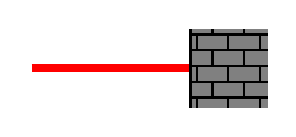
\begin{tikzpicture}
  \wall
  % The "line"
  \draw [red,line width=1mm] (-1,0) -- (1,0);
\end{tikzpicture}
\end{codeexample}

Now we wish to add a blue open arrow tip the red line like, say,
|Stealth[length=1cm,open,blue]|:

现在我们希望向红线添加一个蓝色的开放箭头头部,比如说|Stealth[length=1cm,open,blue]|:
%
\begin{codeexample}[setup code,hidden]
\usetikzlibrary{patterns}
\def\wall{ \fill     [fill=black!50]  (1,-.5) rectangle (2,.5);
           \pattern  [pattern=bricks] (1,-.5) rectangle (2,.5);
           \draw     [line width=1pt]  (1cm+.5pt,-.5) -- ++(0,1); }
\end{codeexample}
\begin{codeexample}[preamble={\usetikzlibrary{arrows.meta}}]
\begin{tikzpicture}
  \wall
  \draw [red,line width=1mm,-{Stealth[length=1cm,open,blue]}]
        (-1,0) -- (1,0);
\end{tikzpicture}
\end{codeexample}

There are several noteworthy things about the blue arrow tip:

关于蓝色箭头头部有几个值得注意的事情:
%
\begin{enumerate}
    \item Notice that the red line no longer goes all the way to the wall.
        Indeed, the red line ends more or less exactly where it meets the
        blue line, leaving the arrow tip empty. Now, recall that the red line
        was supposed to be the path |(-2,0)--(1,0)|; however, this path has
        obviously become much shorter (by 6.25mm to be precise). This effect
        is called \emph{path shortening} in \tikzname.

        注意红线不再一直延伸到墙壁。事实上,红线几乎恰好在遇到蓝线的地方结束,留下了空的箭头头部。现在回想一下,红线应该是路径|(-2,0)--(1,0)|;然而,显然这条路径变得短了很多(准确地说,短了6.25mm)。在\tikzname 中,这种效果被称为\emph{路径缩短}。
    \item The very tip of the arrow just ``touches'' the wall, even we zoom
        out a lot. This point, where the original path ended and where the
        arrow tip should now lie, is called the \emph{tip end} in \tikzname.

        箭头的尖端正好“触碰”墙壁,即使我们将视图缩小很多。在\tikzname 中,原始路径结束的地方,箭头现在应该位于的点被称为\emph{尖端}。
    \item Finally, the point where the red line touches the blue line is the
        point where the original path ``visually ends''. Notice that this is
        not the same as the point that lies at a distance of the arrow's
        |length| from the wall -- rather it lies at a distance of |length|
        minus the |inset|. Let us call this point the \emph{visual
    end} of the arrow.

    最后,红线与蓝线接触的点是原始路径“视觉上结束”的点。请注意,这不是距离箭头的|length|与墙壁之间距离的点,而是距离|length|减去|inset|的距离。我们将这一点称为箭头的\emph{视觉端点}。

\end{enumerate}

As pointed out earlier, for straight lines, shortening the path and rotating
and shifting the arrow tip so that it ends precisely at the tip end and the
visual end lies on a line from the tip end to the start of the line is
relatively easy.

如前所述,对于直线,缩短路径并旋转和移动箭头尖端,使其准确地结束在尖端,并且视觉端点位于从尖端到线段起点的直线上相对较容易。

For curved lines, things are much more difficult and \tikzname\ copes with the
difficulties in different ways, depending on which options you add to arrows.
Here is now a curved red line to which we wish to add our arrow tip (the
original straight red line is shown in light red):

对于曲线,情况要困难得多,\tikzname\ 通过不同的方式处理这些困难,具体取决于您添加到箭头的选项。现在,我们有一条弯曲的红线,我们希望在其中添加箭头(原始的直线示例以浅红色显示):
%
\begin{codeexample}[]
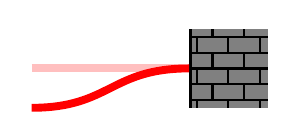
\begin{tikzpicture}
  \wall
  \draw [red!25,line width=1mm] (-1,0) -- (1,0);
  \draw [red,line width=1mm] (-1,-.5) .. controls (0,-.5) and (0,0) .. (1,0);
\end{tikzpicture}
\end{codeexample}

The first way of dealing with curved lines is dubbed the ``quick and dirty''
way (although the option for selecting this option is politely just called
``|quick|'' \dots):

处理曲线的第一种方式被称为“快速且简单”的方式(尽管选择此选项的选项是礼貌地称为“|quick|”……):

\begin{key}{/pgf/arrow keys/quick}
    Recall that curves in \tikzname\ are actually Bézier curves, which means
    that they start and end at certain points and we specify two vectors, one
    for the start and one for the end, that provide tangents to the curve at
    these points. In particular, for the end of the curve, there is a point
    called the \emph{second support point} of the curve such that a tangent to
    the curve at the end goes through this point. In our above example, the
    second support point is at the middle of the light red line and, indeed, a
    tangent to the red line at the point touching the wall is perfectly
    horizontal.

    回想一下,在\tikzname\ 中,曲线实际上是贝塞尔曲线,这意味着它们从某些点开始并结束,并且我们指定两个向量,一个用于起点,一个用于终点,这些向量提供了曲线在这些点处的切线。特别是对于曲线的末端,有一个称为曲线的\emph{第二支撑点}的点,使得曲线在末端的切线通过该点。在上面的示例中,第二支撑点位于浅红色线的中间,并且确实,红线在接触墙壁的点处的切线是完全水平的。

    In order to add our arrow tip to the curved path, our first objective is to
    ``shorten'' the path by 6.25mm. Unfortunately, this is now much more
    difficult than for a straight path. When the |quick| option is added to an
    arrow tip (it is also the default if no special libraries are loaded), we
    cheat somewhat: Instead of really moving along 6.25mm along the path, we
    simply shift the end of the curve by 6.25mm \emph{along the tangent} (which
    is easy to compute). We also have to shift the second support point by the
    same amount to ensure that the line still has the same tangent at the end.
    This will result in the following:
    
    为了在曲线路径上添加箭头尖端,我们的第一个目标是通过6.25mm“缩短”路径。不幸的是,这现在比直线路径困难得多。当将|quick|选项添加到箭头尖端时(如果未加载任何特殊库,则为默认选项),我们有些作弊:我们并不是真正沿着路径移动6.25mm,而是简单地将曲线的末端沿着切线方向平移6.25mm(这很容易计算)。我们还必须将第二支撑点按相同的量平移,以确保线段在末端仍具有相同的切线。这将导致以下结果:
%
\begin{codeexample}[preamble={\usetikzlibrary{arrows.meta}}]
\begin{tikzpicture}
  \wall
  \draw [red!25,line width=1mm] (-1,0) -- (1,0);
  \draw [red,line width=1mm,-{Stealth[length=1cm,open,blue,quick]}]
        (-1,-.5) .. controls (0,-.5) and (0,0) .. (1,0);
\end{tikzpicture}
\end{codeexample}

    They main problem with the above picture is that the red line is no longer
    equal to the original red line (notice much sharper curvature near its
    end). In our example this is not such a bad thing, but it certainly ``not a
    nice thing'' that adding arrow tips to a curve changes the overall shape of
    the curves. This is especially bothersome if there are several similar
    curves that have different arrow heads. In this case, the similar curves
    now suddenly look different.

    上面图片的主要问题是红线不再等于原始红线(注意接近末端的曲率更大)。在我们的示例中,这并不是什么大问题,但是对于添加箭头尖端的曲线来说,改变曲线的整体形状肯定“不好看”。如果存在几个具有不同箭头的类似曲线,这一点尤为麻烦。在这种情况下,类似的曲线突然看起来不同了。

Another big problem with the above approach is that it works only well if
    there is only a single arrow tip. When there are multiple ones, simply
    shifting them along the tangent as the |quick| option does produces
    less-than-satisfactory results:
    
    上述方法的另一个大问题是,它只适用于只有一个箭头尖端的情况。当存在多个箭头尖端时,仅按照|quick|选项所做的方式沿切线移动它们会产生不太令人满意的结果:

\begin{codeexample}[]
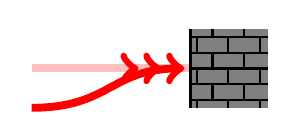
\begin{tikzpicture}
  \wall
  \draw [red!25,line width=1mm] (-1,0) -- (1,0);
  \draw [red,line width=1mm,-{[quick,sep]>>>}]
        (-1,-.5) .. controls (0,-.5) and (0,0) .. (1,0);
\end{tikzpicture}
\end{codeexample}
    %
    Note that the third arrow tip does not really lie on the curve any more.

    请注意,第三个箭头尖端实际上不再位于曲线上。


\end{key}

Because of the shortcomings of the |quick| key, more powerful mechanisms for
shortening lines and rotating arrows tips have been implemented. To use them,
you need to load the following library:

鉴于|quick|选项的缺点,我们实现了更强大的机制来缩短线段和旋转箭头尖端。要使用这些机制,您需要加载以下库:
\begin{tikzlibrary}{bending}
    Load this library to use the |flex|, |flex'|, or |bending| arrow keys. When
    this library is loaded, |flex| becomes the default mode that is used with
    all paths, unless |quick| is explicitly selected for the arrow tip.

    加载此库以使用|flex|、|flex'|或|bending|箭头选项。当加载此库时,|flex|成为所有路径默认使用的模式,除非为箭头尖端显式选择了|quick|选项。
\end{tikzlibrary}

\begin{key}{/pgf/arrow keys/flex=\opt{\meta{factor}} (default 1)}
    When the |bending| library is loaded, this key is applied to all arrow tips
    by default. It has the following effect:
    
    % 加载|bending|库时,默认情况下将此选项应用于所有箭头尖端。它具有以下效果正如前面所指出的,对于直线而言,缩短路径、旋转和移动箭头尖端,使其准确地结束在尖端,并且视觉端点位于从尖端到线段起点的直线上,这是相对容易的。

    当加载|bending|库时,默认情况下将此选项应用于所有箭头尖端。它具有以下效果:
    \begin{enumerate}
        \item Instead of simply shifting the visual end of the arrow along
            the tangent of the curve's end, we really move it along the curve
            by the necessary distance. This operation is more expensive than
            the |quick| operation -- but not \emph{that} expensive, only
            expensive enough so that it is not selected by default for all
            arrow tips. Indeed, some compromises are made in the
            implementation where accuracy was traded for speed, so the
            distance by which the line end is shifted is not necessarily
            \emph{exactly} 6.25mm; only something reasonably close.

            
            与其简单地沿曲线末端的切线移动箭头的视觉端点,我们实际上将其沿曲线移动到必要的距离。这个操作比|quick|操作更昂贵,但并不是\emph{非常}昂贵,只是足够昂贵,以便它不会被默认选择为所有箭头尖端。实际上,在实现过程中做了一些妥协,准确性换取了速度,因此线段末端移动的距离不一定是\emph{精确}的6.25毫米,只是相对接近的数值。



        \item The supports of the line are updated accordingly so that the
            shortened line will still follow \emph{exactly} the original
            line. This means that the curve deformation effect caused by the
            |quick| command does not happen here.

            线段的支撑点相应地更新,以确保缩短后的线段仍然\emph{完全}遵循原始线段。这意味着不会发生由|quick|命令引起的曲线变形效果。


        \item Next, the arrow tip is rotated and shifted as follows: First,
            we shift it so that its tip is exactly at the tip end, where the
            original line ended. Then, the arrow is rotated so the \emph{the
            visual end lies on the line}:

            接下来,箭头尖端按以下方式旋转和移动:首先,我们将其移动到其尖端恰好在原始线段结束位置的位置。然后,箭头被旋转,使得\emph{视觉端点位于线段上}:


            %
\begin{codeexample}[preamble={\usetikzlibrary{arrows.meta,bending}}]
\begin{tikzpicture}
  \wall
  \draw [red!25,line width=1mm] (-1,0) -- (1,0);
  \draw [red,line width=1mm,-{Stealth[length=1cm,open,blue,flex]}]
        (-1,-.5) .. controls (0,-.5) and (0,0) .. (1,0);
\end{tikzpicture}
\end{codeexample}
    \end{enumerate}

    As can be seen in the example, the |flex| option gives a result that is
    visually pleasing and does not deform the path.

    如示例所示,|flex|选项提供了视觉上令人满意且不会扭曲路径的结果。

    There is, however, one possible problem with the |flex| option: The arrow
    tip no longer points along the tangent of the end of the path. This may or
    may not be a problem, put especially for larger arrow tips readers will use
    the orientation of the arrow head to gauge the direction of the tangent of
    the line. If this tangent is important (for example, if it should be
    horizontal), then it may be necessary to enforce that the arrow tip
    ``really points in the direction of the tangent''.

    然而,|flex| 选项可能存在一个问题:箭头尖端不再沿着路径的切线指向。这可能是个问题,尤其对于较大的箭头尖端,读者会使用箭头头部的方向来判断线的切线方向。如果这个切线很重要(例如,如果应该是水平的),那么可能需要强制箭头尖端“真正指向切线的方向”。

    To achieve this, the |flex| option takes an optional \meta{factor}
    parameter, which defaults to |1|. This factor specifies how much the arrow
    tip should be rotated: If set to |0|, the arrow points exactly along a
    tangent to curve at its tip. If set to |1|, the arrow point exactly along a
    line from the visual end point on the curve to the tip. For values in the
    middle, we interpolate the rotation between these two extremes; so
    |flex=.5| will rotate the arrow's visual end ``halfway away from the
    tangent towards the actual position on the line''.
    
    为了实现这一点,|flex| 选项接受一个可选的 \meta{factor} 参数,默认为 |1|。该因子指定箭头尖端应该旋转多少:如果设置为 |0|,箭头恰好沿着曲线在尖端的切线方向。如果设置为 |1|,箭头尖端恰好沿着从曲线上的视觉终点到尖端的直线方向。对于中间的值,我们在这两个极端之间插值旋转;因此,|flex=.5| 将使箭头的视觉终点“从切线方向朝向实际位于直线上的位置的中间位置旋转一半”。
%
\begin{codeexample}[preamble={\usetikzlibrary{arrows.meta,bending}}]
\begin{tikzpicture}
  \wall
  \draw [red!25,line width=1mm] (-1,0) -- (1,0);
  \draw [red,line width=1mm,-{Stealth[length=1cm,open,blue,flex=0]}]
        (-1,-.5) .. controls (0,-.5) and (0,0) .. (1,0);
\end{tikzpicture}
\end{codeexample}
\begin{codeexample}[preamble={\usetikzlibrary{arrows.meta,bending}}]
\begin{tikzpicture}
  \wall
  \draw [red!25,line width=1mm] (-1,0) -- (1,0);
  \draw [red,line width=1mm,-{Stealth[length=1cm,open,blue,flex=.5]}]
        (-1,-.5) .. controls (0,-.5) and (0,0) .. (1,0);
\end{tikzpicture}
\end{codeexample}
    %
    Note how in the above examples the red line is visible inside the open
    arrow tip. Open arrow tips do not go well with a flex value other than~|1|.
    Here is a more realistic use of the |flex=0| key:
    
    请注意,在上述示例中,红线在开放箭头尖端内是可见的。除了 |1| 之外,灵活值与开放箭头尖端不相配。
    这是使用 |flex=0| 选项的更实际的用法:
\begin{codeexample}[preamble={\usetikzlibrary{arrows.meta,bending}}]
\begin{tikzpicture}
  \wall
  \draw [red!25,line width=1mm] (-1,0) -- (1,0);
  \draw [red,line width=1mm,-{Stealth[length=1cm,flex=0]}]
        (-1,-.5) .. controls (0,-.5) and (0,0) .. (1,0);
\end{tikzpicture}
\end{codeexample}
    %
    If there are several arrow tips on a path, the |flex| option positions them
    independently, so that each of them lies optimally on the path:
    
    如果路径上有多个箭头尖端,则 |flex| 选项会独立地将它们定位,使每个箭头尖端都最佳地位于路径上:
\begin{codeexample}[preamble={\usetikzlibrary{bending}}]
\begin{tikzpicture}
  \wall
  \draw [red!25,line width=1mm] (-1,0) -- (1,0);
  \draw [red,line width=1mm,-{[flex,sep]>>>}]
        (-1,-.5) .. controls (0,-.5) and (0,0) .. (1,0);
\end{tikzpicture}
\end{codeexample}
    %
\end{key}

\begin{key}{/pgf/arrow keys/flex'=\opt{\meta{factor}} (default 1)}
    The |flex'| key is almost identical to the |flex| key. The only difference
    is that a factor of |1| corresponds to rotating the arrow tip so that the
    instead of the visual end, the ``ultimate back end'' of the arrow tip lies
    on the red path. In the example instead of having the arrow tip at a
    distance of |6.25mm| from the tip lie on the path, we have the point at a
    distance of |1cm| from the tip lie on the path:
    
    |flex'| 选项与 |flex| 选项几乎完全相同。唯一的区别是,|1| 的因子会将箭头尖端旋转,使箭头尖端的“最终背端”而不是视觉终点位于红色路径上。在这个例子中,箭头尖端与尖端之间的距离为 |6.25mm|,而不是位于路径上的距离为 |1cm| 的点:
\begin{codeexample}[preamble={\usetikzlibrary{arrows.meta,bending}}]
\begin{tikzpicture}
  \wall
  \draw [red!25,line width=1mm] (-1,0) -- (1,0);
  \draw [red,line width=1mm,-{Stealth[length=1cm,open,blue,flex']}]
        (-1,-.5) .. controls (0,-.5) and (0,0) .. (1,0);
\end{tikzpicture}
\end{codeexample}
    %
    Otherwise, the factor works as for |flex| and, indeed |flex=0| and
    |flex'=0| have the same effect.

    否则,因子的工作方式与 |flex| 相同,事实上,|flex=0| 和 |flex'=0| 有相同的效果。

    The main use of this option is not so much with an arrow tip like |Stealth|
    but rather with tips like the standard |>| in the context of a strongly
    curved line:
    
    这个选项的主要用途并不是与 |Stealth| 箭头这样的箭头尖端一起使用,而是与在强烈弯曲的线上的标准 |>| 箭头这样的尖端一起使用:

\begin{codeexample}[preamble={\usetikzlibrary{arrows.meta,bending}}]
\begin{tikzpicture}
  \wall
  \draw [red!25,line width=1mm] (-1,0) -- (1,0);
  \draw [red,line width=1mm,-{Computer Modern Rightarrow[flex]}]
        (0,-.5) .. controls (1,-.5) and (0.5,0) .. (1,0);
\end{tikzpicture}
\end{codeexample}
    %
    In the example, the |flex| option does not really flex the arrow since for
    a tip like the Computer Modern arrow, the visual end is the same as the
    arrow tip -- after all, the red line does, indeed, end almost exactly where
    it used to end.

    在这个例子中,|flex| 选项实际上并没有使箭头弯曲,因为对于像 Computer Modern 箭头这样的尖端,视觉终点与箭头尖端是相同的——毕竟,红线的确几乎正好结束在原来的位置上。

    Nevertheless, you may feel that the arrow tip looks ``wrong'' in the sense
    that it should be rotated. This is exactly what the |flex'| option does
    since it allows us to align the ``back end'' of the tip with the red line:
    
    然而,你可能会觉得箭头尖端在视觉上看起来“不对”,因为它应该被旋转。这正是 |flex'| 选项所做的,因为它允许我们将箭头尖端的“背端”与红线对齐:

\begin{codeexample}[preamble={\usetikzlibrary{arrows.meta,bending}}]
\begin{tikzpicture}
  \wall
  \draw [red!25,line width=1mm] (-1,0) -- (1,0);
  \draw [red,line width=1mm,-{Computer Modern Rightarrow[flex'=.75]}]
        (0,-.5) .. controls (1,-.5) and (0.5,0) .. (1,0);
\end{tikzpicture}
\end{codeexample}
    %
    In the example, I used |flex'=.75| so as not to overpronounce the effect.
    Usually, you will have to fiddle with it sometime to get the ``perfectly
    aligned arrow tip'', but a value of |.75| is usually a good start.

    在这个例子中,我使用了 |flex'=.75|,以免太过强调效果。通常情况下,你需要稍微调整它,以获得“完美对齐的箭头尖端”,但是 |.75| 的值通常是一个很好的开始。
\end{key}

\begin{key}{/pgf/arrow keys/bend}
    \emph{Bending} an arrow tip is a radical solution to the problem of
    positioning arrow tips on a curved line: The arrow tip is no longer
    ``rigid'' but the drawing itself will now bend along the curve. This has
    the advantage that all the problems of flexing with wrong tangents and
    overflexing disappear. The downsides are longer computation times (bending
    an arrow is \emph{much} more expensive that flexing it, let alone than
    quick mode) and also the fact that excessive bending can lead to ugly arrow
    tips. On the other hand, for most arrow tips their bend version are
    visually quite pleasing and create a sophisticated look:
    
    “弯曲”箭头尖端是解决在弯曲线上定位箭头尖端问题的一个激进解决方案:箭头尖端不再“刚性”,而绘图本身现在会沿着曲线弯曲。这有一个优点,即所有与错误切线和过度弯曲相关的问题都消失了。缺点是计算时间更长(弯曲箭头的计算比弯曲箭头要昂贵得多,更不用说快速模式了),而且过度弯曲可能会导致箭头尖端看起来不美观。另一方面,对于大多数箭头尖端来说,它们的弯曲版本在视觉上非常令人愉悦,创造出一种复杂的外观。
\begin{codeexample}[preamble={\usetikzlibrary{arrows.meta,bending}}]
\begin{tikzpicture}
  \wall
  \draw [red!25,line width=1mm] (-1,0) -- (1,0);
  \draw [red,line width=1mm,-{Stealth[length=20pt,bend]}]
        (-1,-.5) .. controls (0,-.5) and (0,0) .. (1,0);
\end{tikzpicture}
\end{codeexample}
\begin{codeexample}[preamble={\usetikzlibrary{bending}}]
\begin{tikzpicture}
  \wall
  \draw [red!25,line width=1mm] (-1,0) -- (1,0);
  \draw [red,line width=1mm,-{[bend,sep]>>>}]
        (-1,-.5) .. controls (0,-.5) and (0,0) .. (1,0);
\end{tikzpicture}
\end{codeexample}
\begin{codeexample}[preamble={\usetikzlibrary{arrows.meta,bending}}]
\begin{tikzpicture}
  \wall
  \draw [red!25,line width=1mm] (-1,0) -- (1,0);
  \draw [red,line width=1mm,-{Stealth[bend,round,length=20pt]}]
        (0,-.5) .. controls (1,-.5) and (0.25,0) .. (1,0);
\end{tikzpicture}
\end{codeexample}
    %
\end{key}
% TODOsp: codeexamples: `bending` library is needed up to here
% TODOsp: codeexamples: `\def\wall` + `patterns` library are needed up to here
% TODOsp: codeexamples: `arrows.meta` library needed up to here


\subsection{Arrow Tip Specifications\\箭头尖端规范}
\label{section-arrow-spec}

\subsubsection{Syntax\\语法}

When you select the arrow tips for the start and the end of a path, you can
specify a whole sequence of arrow tips, each having its own local options. At
the beginning of this section, it was pointed out that the syntax for selecting
the start and end arrow tips is the following:

当选择路径的起始点和终点的箭头尖端时,可以指定一整个序列的箭头尖端,每个尖端都有自己的局部选项。在本节的开头,指出了选择起始点和终点箭头尖端的语法如下:
%
\begin{quote}
    \meta{start specification}|-|\meta{end specification}
\end{quote}

We now have a closer look at what these specifications may look like. The
general syntax of the \meta{start specification} is as follows:

现在我们仔细看看这些规范可能是什么样子的。\meta{start specification} 的一般语法如下:

%
\begin{quote}
    \opt{|[|\meta{options for all tips}|]|} \meta{first arrow tip spec}
    \meta{second arrow tip spec} \meta{third arrow tip spec} \dots
\end{quote}
%
As can be seen, an arrow tip specification may start with some options in
brackets. If this is the case, the \meta{options for all tips} will, indeed, be
applied to all arrow tips that follow. (We will see, in a moment, that there
are even more places where options may be specified and a list of the ordering
in which the options are applied will be given later.)

如您所见,箭头尖端规范可以以方括号中的一些选项开头。如果是这种情况,\meta{options for all tips} 将确实应用于后续的所有箭头尖端。(我们将在一会儿看到,还有更多的地方可以指定选项,下面将给出选项应用的顺序列表。)

The main part of a specification is taken up by a sequence of individual arrow
tip specifications. Such a specification can be of three kinds:

规范的主要部分由一系列单独的箭头尖端规范组成。这样的规范可以有三种形式:
%
\begin{enumerate}
    \item It can be of the form \meta{arrow tip kind
        name}|[|\meta{options}|]|.

        它可以采用形式为\meta{arrow tip kind name}|[|\meta{options}|]|的形式。
    \item It can be of the form \meta{shorthand}|[|\meta{options}|]|.

    它可以采用形式为\meta{shorthand}|[|\meta{options}|]|的形式。
    \item It can be of the form \meta{single char
        shorthand}\opt{|[|\meta{options}|]|}. Note that only for this form
        the brackets are optional.

        它可以采用形式为\meta{single char shorthand}\opt{|[|\meta{options}|]|}的形式。请注意,只有对于这种形式,方括号是可选的。
\end{enumerate}

The easiest kind is the first one: This adds an arrow tip of the kind
\meta{arrow tip kind name} to the sequence of arrow tips with the
\meta{options} applied to it at the start (for the \meta{start specification})
or at the end (for the \meta{end specification}). Note that for the \meta{start
specification} the first arrow tip specified in this way will be at the very
start of the curve, while for the \meta{end specification} the ordering is
reversed: The last arrow tip specified will be at the very end of the curve.
This implies that a specification like

最简单的一种是第一种:在开始(对于\meta{start specification})或结束(对于\meta{end specification})时,将\meta{arrow tip kind name}的箭头尖端添加到箭头尖端序列中,并对其应用\meta{options}。请注意,对于\meta{start specification},以这种方式指定的第一个箭头尖端将位于曲线的起点,而对于\meta{end specification},顺序则相反:指定的最后一个箭头尖端将位于曲线的末端。这意味着像

\begin{quote}
    |Stealth[] Latex[] - Latex[] Stealth[]|
\end{quote}
%
will give perfectly symmetric arrow tips on a line (as one would expect).

这样的规范将在一条线上给出完全对称的箭头尖端(正如人们所期望的)。

It is important that even if there are no \meta{options} for an arrow tip, the
square brackets still need to be written to indicate the end of the arrow tip's
name. Indeed, the opening brackets are used to divide the arrow tip
specification into names.

重要的是,即使箭头尖端没有\meta{options},方括号仍然需要写入,以表示箭头尖端名称的结束。实际上,开放方括号用于将箭头尖端规范分成名称。

Instead of a \meta{arrow tip kind name}, you may also provide the name of a
so-called \emph{shorthand}. Shorthands look like normal arrow tip kind names
and, indeed, you will often be using shorthands without noticing that you do.
The idea is that instead of, say, |Computer Modern Rightarrow| you might wish
to just write |Rightarrow| or perhaps just |To| or even just |>|. For this, you
can create a shorthand that tells \tikzname\ that whenever this shorthand is
used, another arrow tip kind is meant. (Actually, shorthands are somewhat more
powerful, we have a detailed look at them in
Section~\ref{section-arrow-tip-macro}.) For shorthands, the same rules apply as
for normal arrow tip kinds: You \emph{need} to provide brackets so that
\tikzname\ can find the end of the name inside a longer specification.

除了\meta{arrow tip kind name}之外,您还可以提供所谓\emph{shorthand}的名称。Shorthand看起来像普通的箭头尖端名称,实际上,您经常会在不知不觉中使用shorthand。其想法是,您可能希望使用|Computer Modern Rightarrow|而不是直接写|Rightarrow|或者只写|To|,甚至只写|>|。为此,您可以创建一个shorthand,告诉\tikzname,每当使用这个shorthand时,意思是另一种箭头尖端。 (实际上,shorthand的功能更强大,我们在第\ref{section-arrow-tip-macro}节中详细介绍了它们。)对于shorthand,适用与普通箭头尖端相同的规则:您需要提供方括号,以便\tikzname\ 可以找到较长规范中名称的结束。

The third kind of arrow tip specifications consist of just a single letter like
|>| or |)| or |*| or even |o| or |x| (but you may not use |[|, |]|, or |-|
since they will confuse the parser). These single letter arrow specifications
will invariably be shorthands that select some ``real'' arrow tip instead. An
important feature of single letter arrow tips is that they do \emph{not} need
to be followed by options (but they may).

第三种箭头尖端规范仅由单个字母组成,例如|>|或|)|或|*|甚至|o|或|x|(但不能使用|[|、|]|或|-|,因为它们会使解析器混淆)。这些单个字母箭头规范无疑是选择某个“真实”箭头尖端的shorthand。单个字母箭头尖端的一个重要特点是它们\emph{不需要}后面跟随选项(但可以有)。

Now, since we can use any letter for single letter shorthands, how can
\tikzname\ tell whether by |foo[]| we mean an arrow tip kind |foo| without any
options or whether we mean an arrow tip called |f|, followed by two arrow tips
called |o|? Or perhaps an arrow tip called |f| followed by an arrow tip called
|oo|? To solve this problem, the following rule is used to determine which of
the three possible specifications listed above applies: First, we check whether
everything from the current position up to the next opening bracket (or up to
the end) is the name of an arrow tip or of a shorthand. In our case, |foo|
would first be tested under this rule. Only if |foo| is neither the name of an
arrow tip kind nor of a shorthand does \tikzname\ consider the first letter of
the specification, |f| in our case. If this is not the name of a shorthand, an
error is raised. Otherwise the arrow tip corresponding to |f| is added to the
list of arrow tips and the process restarts with the rest. Thus, we would next
text whether |oo| is the name of an arrow tip or shorthand and, if not, whether
|o| is such a name.

现在,由于我们可以使用任何字母作为单个字母shorthand,\tikzname\ 如何判断|foo[]|是指没有任何选项的箭头尖端|foo|,还是指名为|f|的箭头尖端,后跟两个名为|o|的箭头尖端?或者是一个名为|f|的箭头尖端,后跟一个名为|oo|的箭头尖端?为了解决这个问题,使用以下规则来确定上述三种可能的规范中的哪一种适用:首先,我们检查从当前位置到下一个开括号(或到结尾)的所有内容是否是箭头尖端或shorthand的名称。在我们的情况下,|foo|将首先根据此规则进行测试。只有当|foo|既不是箭头尖端的名称,也不是shorthand的名称时,\tikzname\ 才会考虑规范的第一个字母,即我们的例子中的|f|。如果它不是shorthand的名称,将引发错误。否则,与|f|对应的箭头尖端将添加到箭头尖端列表中,并重新开始这个过程。因此,我们接下来将测试|oo|是否是箭头尖端或shorthand的名称,如果不是,则测试|o|是否是这样的名称。

All of the above rules mean that you can rather easily specify arrow tip
sequences if they either mostly consist of single letter names or of longer
names. Here are some examples:

上述所有规则意味着,如果箭头尖端序列主要由单个字母名称或较长名称组成,您可以相当容易地指定它们。以下是一些例子:
%
\begin{itemize}
    \item |->>>| is interpreted as three times the |>| shorthand since |>>>| is
        not the name of any arrow tip kind (and neither is |>>|).

        |->>>|被解释为三次使用|>|shorthand,因为|>>>|既不是任何箭头尖端名称的名称(|>>|也不是)。
    \item |->[]>>| has the same effect as the above.

    |->[]>>|具有与上述相同的效果。
    \item |-[]>>>| also has the same effect.

    |-[]>>>|也具有相同的效果。
    \item |->[]>[]>[]| so does this.

    |->[]>[]>[]|也是如此。
    \item |->Stealth| yields an arrow tip |>| followed by a |Stealth| arrow
        at the end.

        |->Stealth|产生一个以|>|开头的箭头尖端,后跟一个|Stealth|箭头在末尾。
    \item |-Stealth>| is illegal since there is no arrow tip |Stealth>| and
        since |S| is also not the name of any arrow tip.

        |-Stealth>|是不合法的,因为没有名为|Stealth>|的箭头尖端,而且|S|也不是任何箭头尖端的名称。
    \item |-Stealth[] >| is legal and does what was presumably meant in the
        previous item.

        |-Stealth[] >|是合法的,并且做了之前的项目中可能意味着的事情。
    \item |< Stealth-| is legal and is the counterpart to |-Stealth[] >|.

    |< Stealth-|是合法的,并且是|-Stealth[] >|的对应物。
    \item |-Stealth[length=5pt] Stealth[length=6pt]| selects two stealth
        arrow tips, but at slightly different sizes for the end of lines.

        |-Stealth[length=5pt] Stealth[length=6pt]|选择了两个隐形箭头尖端,但大小略有不同,用于线的末端。
\end{itemize}

An interesting question concerns how flexing and bending interact with multiple
arrow tips: After all, flexing and quick mode use different ways of shortening
the path so we cannot really mix them. The following rule is used: We check,
independently for the start and the end specifications, whether at least one
arrow tip in them uses one of the options |flex|, |flex'|, or |bend|. If so,
all |quick| settings in the other arrow tips are ignored and treated as if
|flex| had been selected for them, too.

有一个有趣的问题与弯曲和弯曲如何与多个箭头尖端交互有关:毕竟,弯曲和快速模式使用不同的路径缩短方式,因此我们不能真正混合它们。使用以下规则:独立地对起始和结束规范进行检查,看它们中是否至少有一个箭头尖端使用了|flex|、|flex'|或|bend|选项。如果是这样,那么其他箭头尖端中的所有|quick|设置将被忽略,并且被视为如果也为它们选择了|flex|。


\subsubsection{Specifying Paddings\\指定填充}

When you provide several arrow tips in a row, all of them are added to the
start or end of the line:

当您在一行中指定多个箭头尖端时,它们全部添加到该行的起始或结束处:
\begin{codeexample}[]
\tikz \draw [<<<->>>>] (0,0) -- (2,0);
\end{codeexample}
%
The question now is what will be the distance between them? For this, the
following arrow key is important:

现在的问题是它们之间的距离将是多少?为此,以下箭头键很重要:

\begin{key}{/pgf/arrow keys/sep=\meta{dimension}| |\opt{\meta{line
    width factor}}| |\opt{\meta{outer factor}} (default 0.88pt .3 1)%
}
    When a sequence of arrow tips is specified in an arrow tip specification
    for the end of the line, the arrow tips are normally arranged in such a way
    that the tip of each arrow ends exactly at the ``back end'' of the next
    arrow tip (for start specifications, the ordering is inverted, of course).
    Now, when the |sep| option is set, instead of exactly touching the back end
    of the next arrow, the specified \meta{dimension} is added as additional
    space (the distance may also be negative, resulting in an overlap of the
    arrow tips). The optional factors have the same meaning as for the |length|
    key, see that key for details.

    当在箭头尖端规范中为行尾指定了一系列箭头尖端时,通常会按照这样的方式排列箭头尖端,使得每个箭头的尖端恰好在下一个箭头尖端的“后端”结束(对于起始规范,顺序是相反的)。现在,当设置了|sep|选项时,指定的\meta{dimension}将作为额外空间添加,而不是与下一个箭头的后端恰好接触(距离也可以是负值,导致箭头尖端重叠)。可选的因子与|length|键具有相同的含义,请参阅该键以了解详细信息。

    Let us now have a look at some examples. First, we use two arrow tips with
    different separations between them:
    
    现在让我们来看一些例子。首先,我们使用两个具有不同间隔的箭头尖端:

\begin{codeexample}[preamble={\usetikzlibrary{arrows.meta}}]
\tikz {
  \draw [-{>[sep=1pt]>[sep= 2pt]>}] (0,1.0) -- (1,1.0);
  \draw [-{>[sep=1pt]>[sep=-2pt]>}] (0,0.5) -- (1,0.5);
  \draw [-{>         >[sep]     >}] (0,0.0) -- (1,0.0);
}
\end{codeexample}

    You can also specify a |sep| for the last arrow tip in the sequence (for
    end specifications, otherwise for the first arrow tip). In this case, this
    first arrow tip will not exactly ``touch'' the point where the path ends,
    but will rather leave the specified amount of space. This is usually quite
    desirable.
    
    您还可以为序列中的最后一个箭头尖端(对于结束规范)或第一个箭头尖端(对于起始规范)指定|sep|。在这种情况下,第一个箭头尖端将不会与路径结束的点“接触”,而是留下指定的空间量。这通常非常理想。

\begin{codeexample}[preamble={\usetikzlibrary{arrows.meta,positioning}}]
\tikz {
  \node [draw] (A) {A};
  \node [draw] (B) [right=of A] {B};

  \draw [-{>>[sep=2pt]}] (A) to [bend left=45] (B);
  \draw [- >>          ] (A) to [bend right=45] (B);
}
\end{codeexample}
    %
    Indeed, adding a |sep| to an arrow tip is \emph{very} desirable, so you
    will usually write something like |>={To[sep]}| somewhere near the start of
    your files.

    事实上,为箭头尖端添加|sep|非常理想,因此您通常会在文件的开头附近写入类似于|>={To[sep]}|的内容。

    One arrow tip kind can be quite useful in this context: The arrow tip kind
    |_|. It draws nothing and has zero length, \emph{but} it has |sep| set as a
    default option. Since it is a single letter shorthand, you can write short
    and clean ``code'' in this way:
    
    在这种情况下,一种箭头尖端非常有用:箭头尖端||。它不绘制任何内容,并且长度为零,\emph{但是}它默认设置了|sep|选项。由于它是一个单字母缩写,因此您可以以简短而干净的方式编写“代码”:
\begin{codeexample}[]
\tikz \draw [->_>] (0,0) -- (1,0);
\end{codeexample}
\begin{codeexample}[]
\tikz \draw [->__>] (0,0) -- (1,0);
\end{codeexample}
    %
    However, using the |sep| option will be faster than using the |_| arrow tip
    and it also allows you to specify the desired length directly.

    但是,使用|sep|选项比使用||箭头尖端更快,而且还允许您直接指定所需的长度。
\end{key}


\subsubsection{Specifying the Line End\\指定线的结束}

In the previous examples of sequences of arrow tips, the line of the path
always ended at the last of the arrow tips (for end specifications) or at the
first of the arrow tips (for start specifications). Often, this is what you may
want, but not always. Fortunately, it is quite easy to specify the desired end
of the line: The special single char shorthand |.| is reserved to indicate that
last arrow that is still part of the line; in other words, the line will stop
at the last arrow before |.| is encountered (for end specifications) are at the
first arrow following |.| (for start specifications).

在前面的箭头尖端序列示例中,路径的线始终在箭头尖端的最后结束(对于结束规范)或在箭头尖端的第一个结束(对于起始规范)。通常情况下,这可能是您想要的,但并非总是如此。幸运的是,很容易指定线的期望结束:特殊的单字符简写|.|保留用于指示仍然是线一部分的最后一个箭头;换句话说,线将在遇到|.|之前的最后一个箭头处停止(对于结束规范),或在|.|后面的第一个箭头处停止(对于起始规范)。

\begin{codeexample}[]
\tikz [very thick] \draw [<<<->>>] (0,0) -- (2,0);
\end{codeexample}
\begin{codeexample}[]
\tikz [very thick] \draw [<.<<->.>>] (0,0) -- (2,0);
\end{codeexample}
\begin{codeexample}[]
\tikz [very thick] \draw [<<.<-.>>>] (0,0) -- (2,0);
\end{codeexample}
\begin{codeexample}[]
\tikz [very thick] \draw [<<.<->.>>] (0,0) to [bend left] (2,0);
\end{codeexample}

It is permissible that there are several dots in a specification, in this case
the first one ``wins'' (for end specifications, otherwise the last one).

允许在规范中有几个点,这种情况下允许有多个点在规范中,此时第一个点为准(对于结束规范而言),否则为最后一个点。

Note that |.| is parsed as any other shorthand. In particular, if you wish to
add a dot after a normal arrow tip kind name, you need to add brackets:

注意,|.|与其他简写一样进行解析。特别是,如果您希望在普通箭头尖端名称后添加一个点,您需要添加括号:

\begin{codeexample}[preamble={\usetikzlibrary{arrows.meta}}]
\tikz [very thick] \draw [-{Stealth[] . Stealth[] Stealth[]}] (0,0) -- (2,0);
\end{codeexample}
%
Adding options to |.| is permissible, but they have no effect. In particular,
|sep| has no effect since a dot is not an arrow.

对|.|添加选项是允许的,但它们没有任何效果。特别是,|sep|没有效果,因为点不是箭头。


\subsubsection{Defining Shorthands\\定义简写}
\label{section-arrow-tip-macro}

It is often desirable to create ``shorthands'' for the names of arrow tips that
you are going to use very often. Indeed, in most documents you will only need a
single arrow tip kind and it would be useful that you could refer to it just as
|>| in your arrow tip specifications. As another example, you might constantly
wish to switch between a filled and a non-filled circle as arrow tips and would
like to use |*| and |o| are shorthands for these case. Finally, you might just
like to shorten a long name like |Computer Modern Rightarrow| down to just, say
|To| or something similar.

通常希望为您经常使用的箭头尖端名称创建“简写”是很有用的。实际上,在大多数文档中,您只需要一个箭头尖端类型,并且可以在箭头尖端规范中将其表示为|>|。另一个例子是,您可能经常希望在填充和非填充的圆圈之间切换作为箭头尖端,并且希望使用|*|和|o|作为这些情况的简写。最后,您可能只想将长名称如|Computer Modern Rightarrow|缩短为,比如|To|或类似的名称。

All of these case can be addressed by defining appropriate shorthands. This is
done using the following handler:

所有这些情况都可以通过定义适当的简写来解决。可以使用以下处理程序来完成:

\begin{handler}{{.tip}{=\meta{end specification}}}
    Defined the \meta{key} as a name that can be used inside arrow tip
    specifications. If the \meta{key} has a path before it, this path is
    ignored (so there is only one ``namespace'' for arrow tips). Whenever it is
    used, it will be replaced by the \meta{end specification}. Note that you
    must \emph{always} provide (only) an end specification; when the \meta{key}
    is used inside a start specification, the ordering and the meaning of the
    keys inside the \meta{end specification} are translated automatically.
    \todosp{remaining instance of bug \#473}

    将\meta{key}定义为在箭头尖端规范中使用的名称。如果\meta{key}之前有路径,则忽略该路径(因此箭头尖端只有一个“命名空间”)。每当使用该\meta{key}时,它将被\meta{end specification}替换。请注意,您必须始终提供(仅)一个结束规范;当在起始规范内使用\meta{key}时,\meta{end specification}中的键的顺序和含义会自动转换。
    %
\begin{codeexample}[preamble={\usetikzlibrary{arrows.meta}}]
\tikz [foo /.tip = {Stealth[sep]. >>}]
  \draw [-foo] (0,0) -- (2,0);
\end{codeexample}
\begin{codeexample}[preamble={\usetikzlibrary{arrows.meta}}]
\tikz [foo /.tip = {Stealth[sep] Latex[sep]},
       bar /.tip = {Stealth[length=10pt,open]}]
  \draw [-{foo[red] . bar}] (0,0) -- (2,0);
\end{codeexample}

    In the last of the examples, we used |foo[red]| to make the arrows red. Any
    options given to a shorthand upon use will be passed on to the actual
    arrows tip for which the shorthand stands. Thus, we could also have written
    |Stealth[sep,red]| |Latex[sep,red]| instead of |foo[red]|. In other words,
    the ``replacement'' of a shorthand by its ``meaning'' is a semantic
    replacement rather than a syntactic replacement. In particular, the
    \meta{end specification} will be parsed immediately when the shorthand is
    being defined. However, this applies only to the options inside the
    specification, whose values are evaluated immediately. In contrast, which
    actual arrow tip kind is meant by a given shorthand used inside the
    \meta{end specification} is resolved only up each use of the shorthand.
    This means that when you write
    
    在最后一个示例中,我们使用|foo[red]|使箭头变为红色。在使用简写时,给定的任何选项都将传递给简写所代表的实际箭头尖端。因此,我们也可以写成|Stealth[sep,red]| |Latex[sep,red]|而不是|foo[red]|。换句话说,简写的“替代”是语义替代,而不是语法替代。特别地,当定义简写时,\meta{end specification}将立即解析。然而,这仅适用于规范内部的选项,其值会立即评估。相反,给定简写在\meta{end specification}内表示的实际箭头尖端种类是根据每次使用简写进行解析的。这意味着当您编写时


    \begin{quote}
        |dup /.tip = >>|
    \end{quote}
    %
    and then later write

    然后稍后写

    %
    \begin{quote}
        |> /.tip = whatever|
    \end{quote}
    %
    then |dup| will have the effect as if you had written
    |whatever[]whatever[]|. You will find that this behavior is what one would
    expect.

    那么 |dup| 的效果就相当于你写了
    |whatever[]whatever[]|。你会发现这个行为是符合预期的。



    There is one problem we have not yet addressed: The asymmetry of single
    letter arrow tips like |>| or |)|. When someone writes
    
    还有一个问题我们还没有解决:单个字母箭头标记的不对称性,比如 |>| 或者 |)|。当有人写下面的内容时:
\begin{codeexample}[]
\tikz \draw [<->] (0,0) -- (1,0);
\end{codeexample}
    %
    we rightfully expect one arrow tip pointing left at the left end and an
    arrow tip pointing right at the right end. However, compare
    
    我们合理地期望箭头标记在左端指向左,右端指向右。然而,比较下面两种情况:
\begin{codeexample}[]
\tikz \draw [>->] (0,0) -- (1,0);
\end{codeexample}
\begin{codeexample}[preamble={\usetikzlibrary{arrows.meta}}]
\tikz \draw [Stealth-Stealth] (0,0) -- (1,0);
\end{codeexample}
    %
    In both cases, we have \emph{identical} text in the start and end
    specifications, but in the first case we rightfully expect the left arrow
    to be flipped.

    在这两种情况下,起始和结束的规范中的文本是\emph{相同的},但是在第一种情况下我们合理地期望左箭头被翻转。

    The solution to this problem is that it is possible to define two names for
    the same arrow tip, namely one that is used inside start specifications and
    one for end specifications. Now, we can decree that the ``name of |>|''
    inside start specifications is simply |<| and the above problems disappear.

    解决这个问题的方法是可以为同一个箭头标记定义两个名称,一个用于起始规范,一个用于结束规范。现在,我们可以规定在起始规范中使用的 ``|>| 的名称'' 简单地是 |<|,这样上述问题就消失了。

To specify different names for a shorthand in start and end specifications,
    use the following syntax: Instead of \meta{key}, you use \meta{name in
    start specifications}|-|\meta{name in end specifications}. Thus, to set the
    |>| key correctly, you actually need to write
    
    要在起始规范和结束规范中为缩写指定不同的名称,使用以下语法:用 \meta{name in start specifications}|-|\meta{name in end specifications} 替代 \meta{key}。因此,要正确设置 |>| 键,实际上需要写成:

\begin{codeexample}[preamble={\usetikzlibrary{arrows.meta}}]
\tikz [<-> /.tip = Stealth] \draw [<->>] (0,0) -- (1,0);
\end{codeexample}
\begin{codeexample}[preamble={\usetikzlibrary{arrows.meta}}]
\tikz [<-> /.tip = Latex] \draw [>-<] (0,0) -- (1,0);
\end{codeexample}

    Note that the above also works even though we have not set |<| as an arrow
    tip name for end specifications! The reason this works is that the
    \tikzname\ (more precisely, \pgfname) actually uses the following
    definition internally:

    请注意,即使我们没有将 |<| 设置为结束规范的箭头标记名称,上述方法也能起作用!这样能够起作用的原因是 \tikzname(更准确地说,\pgfname )在内部实际上使用了以下定义:

    %
    \begin{quote}
        |>-< /.tip = >[reversed]|
    \end{quote}
    %
    Translation: ``When |<| is used in an end specification, please replace it
    by |>|, but reversed. Also, when |>| is used in a start specification, we
    also mean this inverted |>|.''

    翻译:“当在结束规范中使用 |<| 时,请将其替换为 |>|,但是翻转。同样,当在起始规范中使用 |>| 时,我们也是指这个翻转过的 |>|。”


    By default, |>| is a shorthand for |To| and |To| is a shorthand for |to|
    (an arrow from the old libraries) when |arrows.meta| is not loaded library.
    When |arrows.meta| is loaded, |To| is redefined to mean the same as
    |Computer Modern Rightarrow|.

    默认情况下,|>| 是 |To| 的简写,而 |To| 是当未加载 |arrows.meta| 库时的 |to|(旧库中的箭头)的简写。当加载了 |arrows.meta| 时,|To| 被重新定义为与 |Computer Modern Rightarrow| 相同的意思。

\end{handler}

\begin{key}{/tikz/>=\meta{end arrow specification}}
    This is a short way of saying |<->/.tip=|\meta{end arrow specification}.
    
    这是一种简化的方式,即 |<->/.tip=|\meta{end arrow specification}。
\begin{codeexample}[preamble={\usetikzlibrary{arrows.meta}}]
\begin{tikzpicture}[scale=2,ultra thick]
  \begin{scope}[>=Latex]
    \draw[>->]    (0pt,3ex) -- (1cm,3ex);
    \draw[|<->>|] (0pt,2ex) -- (1cm,2ex);
  \end{scope}
  \begin{scope}[>=Stealth]
    \draw[>->]    (0pt,1ex) -- (1cm,1ex);
    \draw[|<<.<->|] (0pt,0ex) -- (1cm,0ex);
  \end{scope}
\end{tikzpicture}
\end{codeexample}
    %
\end{key}

\begin{key}{/tikz/shorten <=\meta{length}}
    Shorten the path by \meta{length} in the direction of the starting point.

    在起始点方向上将路径缩短 \meta{length}。


\end{key}

\begin{key}{/tikz/shorten >=\meta{length}}
    Shorten the path by \meta{length} in the direction of the end point.

    在结束点方向上将路径缩短 \meta{length}。
\end{key}


\subsubsection{Scoping of Arrow Keys\\箭头键的作用域}
\label{section-arrow-scopes}

There are numerous places where you can specify keys for an arrow tip. There
is, however, one final place that we have not yet mentioned:

有许多地方可以为箭头标记指定键。然而,还有一个我们还没有提到的最后一个地方:

\begin{key}{/tikz/arrows=|[|\meta{arrow keys}|]|}
    The |arrows| key, which is normally used to set the arrow tips for the
    current scope, can also be used to set some arrow keys for the current
    scope. When the argument to |arrows| starts with an opening bracket and
    only otherwise contains one further closing bracket at the very end, this
    semantic of the |arrow| key is assumed.

    |arrows| 键通常用于设置当前作用域的箭头标记,也可以用于为当前作用域设置一些箭头键。当 |arrows| 的参数以一个开放括号开头,并且只在最后一个位置包含一个闭合括号时,就假设 |arrow| 键的语义如此。

    The \meta{arrow keys} will be set for the rest of current scope. This is
    useful for generally setting some design parameters or for generally
    switching on, say, bending as in:

    \meta{arrow keys} 将在当前作用域的剩余部分设置。这对于通常设置一些设计参数或通常打开弯曲等非常有用,如:

    %
\begin{codeexample}[code only]
\tikz [arrows={[bend]}] ... % Bend all arrows
\end{codeexample}
    %
\end{key}

We can now summarize which arrow keys are applied in what order when an arrow
tip is used:

现在我们可以总结当使用箭头标记时,应用哪些箭头键以及它们的顺序:
%
\begin{enumerate}
    \item First, the so-called \emph{defaults} are applied, which are values
        for the different parameters of a key. They are fixed in the
        definition of the key and cannot be changed. Since they are executed
        first, they are only the ultimate fallback.

        首先,应用所谓的\emph{默认值},它们是键的不同参数的值。它们在键的定义中固定且无法更改。由于它们首先执行,它们只是最终的后备。


    \item The \meta{keys} from the use of |arrows=[|\meta{keys}|]| in all
        enclosing scopes.

        在所有包围作用域中使用 |arrows=[|\meta{keys}|]| 时的 \meta{keys}。


    \item Recursively, the \meta{keys} provided with the arrow tip inside
        shorthands.

        递归地,用于缩写内部的箭头标记提供的 \meta{keys}。


    \item The keys provided at the beginning of an arrow tip specification in
        brackets.

        在规范中的箭头标记规范开始处提供的键。


    \item The keys provided directly next to the arrow tip inside the
        specification.

        在规范中箭头标记旁边直接提供的键。


\end{enumerate}


\subsection{Reference: Arrow Tips\\参考:箭头标记}
\label{section-arrows-meta}

\begin{pgflibrary}{arrows.meta}
    This library defines a large number of standard ``meta'' arrow tips.
    ``Meta'' means that you can configure these arrow tips in many different
    ways like changing their size or their line caps and joins and many other
    details.

    该库定义了大量标准的“元”箭头标记。
    “元”表示您可以以许多不同的方式配置这些箭头标记,例如更改它们的大小、线帽和连接方式以及许多其他细节。


    The only reason this library is not loaded by default is for compatibility
    with older versions of \tikzname. You can, however, safely load and use
    this library alongside the older libraries |arrows| and |arrows.spaced|.

    这个库不默认加载的唯一原因是为了与旧版本的\tikzname 兼容。然而,你可以安全地加载和使用这个库以及旧的库|arrows|和|arrows.spaced|。
\end{pgflibrary}

The different arrow tip kinds defined in the |arrows.meta| library can be
classified in different groups:

在|arrows.meta|库中定义的不同箭头类型可以分为不同的组:

%
\begin{itemize}
    \item \emph{Barbed} arrow tips consist mainly of lines that ``point
        backward'' from the tip of the arrow and which are not filled. For
        them, filling has no effect. A typical example is \tikz [baseline]
        \draw (0,.5ex) -- (1.5em,.5ex) [-Straight Barb];. Here is the list of
        defined arrow tips:

        \emph{Barbed} 箭头主要由从箭头尖端“向后指”的线组成,这些线没有填充。对于这些箭头,填充没有效果。一个典型的例子是\tikz [baseline]\draw (0,.5ex) -- (1.5em,.5ex) [-Straight Barb];。以下是定义的箭头列表:
        %
        \begin{arrowexamples}
            \arrowexample Arc Barb[]
            \arrowexample Bar[]
            \arrowexample Bracket[]
            \arrowexample Hooks[]
            \arrowexample Parenthesis[]
            \arrowexample Straight Barb[]
            \arrowexample Tee Barb[]
        \end{arrowexamples}

        All of these arrow tips can be configured and resized in many different
        ways as described in the following. Above, they are shown at their
        ``natural'' sizes, which are chosen in such a way that for a line width
        of 0.4pt their width matches the height of a letter ``x'' in Computer
        Modern at 11pt (with some ``overshooting'' to create visual
        consistency).

        所有这些箭头都可以以多种不同的方式进行配置和调整大小,如下所述。上面显示的是它们的“自然”大小,这样选择的宽度使得在0.4pt的线宽下,它们的宽度与11pt的计算机现代字体中的字母“x”的高度相匹配(为了创建视觉上的一致性,有些“超调”)。


    \item \emph{Mathematical} arrow tips are actually a subclass of the
        barbed arrow tips, but we list them separately. They contain arrow
        tips that look exactly like the tips of arrows used in mathematical
        fonts such as the |\to|-symbol $\to$ from standard \TeX.
        
        \emph{Mathematical} 箭头实际上是 barbed 箭头的一个子类,但我们单独列出它们。它们包含的箭头看起来与数学字体(如标准\TeX 中的|\to|符号$\to$)中使用的箭头相同。

        \begin{arrowexamples}
            \arrowexample Classical TikZ Rightarrow[]
            \arrowexample Computer Modern Rightarrow[]
            \arrowexampledouble Implies[]
            \arrowexample To[]
        \end{arrowexamples}
        %
        The |To| arrow tip is a shorthand for |Computer Modern Rightarrow| when
        |arrows.meta| is loaded.

        当加载|arrows.meta|时,|To| 箭头是 |Computer Modern Rightarrow| 的简写。
    \item \emph{Geometric} arrow tips consist of a filled shape like a kite
        or a circle or a ``stealth-fighter-like'' shape. A typical example is
        \tikz [baseline] \draw (0,.5ex) -- (1.5em,.5ex) [-Stealth];. These
        arrow tips can also be used in an ``open'' variant as in \tikz
        [baseline] \draw (0,.5ex) -- (1.5em,.5ex) [-{Stealth[open]}];.
        %

        \emph{Geometric} 箭头由填充的形状组成,如风筝、圆圈或“隐身战斗机”形状。一个典型的例子是\tikz [baseline]\draw (0,.5ex) -- (1.5em,.5ex) [-Stealth];。这些箭头也可以用“开放”变体使用,如\tikz [baseline]\draw (0,.5ex) -- (1.5em,.5ex) [-{Stealth[open]}];。以下是“开放”变体:

        \begin{arrowexamples}
            \arrowexample Circle[]
            \arrowexample Diamond[]
            \arrowexample Ellipse[]
            \arrowexample Kite[]
            \arrowexample Latex[]
            \arrowexample Latex[round]
            \arrowexample Rectangle[]
            \arrowexample Square[]
            \arrowexample Stealth[]
            \arrowexample Stealth[round]
            \arrowexample Triangle[]
            \arrowexample Turned Square[]
        \end{arrowexamples}

        Here are the ``open'' variants:
        %
        \begin{arrowexamples}
            \arrowexample Circle[open]
            \arrowexample Diamond[open]
            \arrowexample Ellipse[open]
            \arrowexample Kite[open]
            \arrowexample Latex[open]
            \arrowexample Latex[round,open]
            \arrowexample Rectangle[open]
            \arrowexample Square[open]
            \arrowexample Stealth[open]
            \arrowexample Stealth[round,open]
            \arrowexample Triangle[open]
            \arrowexample Turned Square[open]
        \end{arrowexamples}

        Note that ``open'' arrow tips are not the same as ``filled with
        white'', which is also available (just say |fill=white|). The
        difference is that the background will ``shine through'' an open
        arrow, while a filled arrow always obscures the background:
        
        注意,“开放”箭头与“填充为白色”的箭头不同,后者也可用(只需添加|fill=white|)。区别在于背景会“透过”开放的箭头,而填充的箭头总是遮挡背景。
\begin{codeexample}[preamble={\usetikzlibrary{arrows.meta}}]
\tikz {
  \shade [left color=white, right color=red!50] (0,0) rectangle (4,1);

  \draw [ultra thick,-{Triangle[open]}]       (0,2/3) -- ++ (3,0);
  \draw [ultra thick,-{Triangle[fill=white]}] (0,1/3) -- ++ (3,0);
}
\end{codeexample}

    \item \emph{Cap} arrow tips are used to add a ``cap'' to the end of a
        line. The graphic languages underlying \tikzname\ (\textsc{pdf},
        \textsc{postscript} or \textsc{svg}) all support three basic types of
        line caps on a very low level: round, rectangular, and ``butt''.
        Using cap arrow tips, you can add new caps to lines and use different
        caps for the end and the start. An example is the line \tikz
        [baseline] \draw [line width=1ex, {Round Cap[reversed]}-{Triangle
        Cap[] . Fast Triangle[] Fast Triangle[]}] (0,0.5ex) -- (2em,0.5ex);.
        %

        \emph{Cap} 箭头用于在线的末端添加“帽子”。\tikz [baseline]\draw [line width=1ex, {Round Cap[reversed]}-{Triangle Cap[] . Fast Triangle[] Fast Triangle[]}] (0,0.5ex) -- (2em,0.5ex); 是一个示例。

        \begin{arrowcapexamples}
            \arrowcapexample Butt Cap[]
            \arrowcapexample Fast Round[]
            \arrowcapexample Fast Triangle[]
            \arrowcapexample Round Cap[]
            \arrowcapexample Triangle Cap[]
        \end{arrowcapexamples}
    \item \emph{Special} arrow tips are used for some specific purpose and do
        not fit into the above categories.
        
        \emph{Special} 箭头用于某些特定目的,不适用于上述类别。


        \begin{arrowexamples}
            \arrowexample Rays[]
            \arrowexample Rays[n=8]
        \end{arrowexamples}
\end{itemize}


\subsubsection{Barbed Arrow Tips}

\begin{arrowtip}{Arc Barb}{
    This arrow tip attaches an arc to the end of the line whose angle is given
    by the |arc| option. The |length| and |width| parameters refer to the size
    of the arrow tip for |arc| set to 180 degrees, which is why in the example
    for |arc=210| the actual length is larger than the specified |length|. The
    line width is taken into account for the computation  of the length and
    width. Use the |round| option to add round caps to the end of the arcs.

    这种箭头将一个弧附加到线的末端,其角度由|arc|选项给出。|length|和|width|参数是针对|arc|设置为180度时箭头尺寸的参考,这就是为什么在|arc=210|的示例中,实际长度大于指定的|length|。线的线宽被考虑在内,用于计算长度和宽度。使用|round|选项可以在弧的末端添加圆角帽。
}%
{length=1.5cm,arc=210}%
{length=1.5cm,width=3cm}

    \begin{arrowexamples}
        \arrowexample[]
        \arrowexampledup[sep]
        \arrowexampledupdot[sep]
        \arrowexample[arc=120]
        \arrowexample[arc=270]
        \arrowexample[length=2pt]
        \arrowexample[length=2pt,width=5pt]
        \arrowexample[line width=2pt]
        \arrowexample[reversed]
        \arrowexample[round]
        \arrowexample[slant=.3]
        \arrowexample[left]
        \arrowexample[right]
        \arrowexample[harpoon,reversed]
        \arrowexample[red]
    \end{arrowexamples}
    %
    The following options have no effect: |open|, |fill|.

    以下选项没有效果:|open|、|fill|。



    On |double| lines, the arrow tip will not look correct.

    在|double|线上,箭头看起来不正确。


\end{arrowtip}

\begin{arrowtipsimple}{Bar}
    A simple bar. This is a simple instance of |Tee Barb| for length zero.

    一个简单的条。这是|Tee Barb|的一个长度为零的简单实例。


\end{arrowtipsimple}

\begin{arrowtip}{Bracket}{
    This is an instance of the |Tee Barb| \todosp{no space shown here} arrow tip that results in something
    resembling a bracket. Just like the |Parenthesis| arrow tip, a |Bracket| is
    not modelled from a text square bracket, but rather its size has been
    chosen so that it fits with the other arrow tips.

    这是|Tee Barb|\todosp{此处没有显示空格}箭头的一个实例,看起来像一个括号。与|Parenthesis|箭头一样,|Bracket|也不是从文本方括号模拟出来的,该库不被默认加载的唯一原因是为了与旧版本的\tikzname 兼容。然而,你可以安全地加载和使用该库以及旧版库|arrows|和|arrows.spaced|。


}%
{}%
{}

    \begin{arrowexamples}
        \arrowexample[]
        \arrowexampledup[sep]
        \arrowexampledupdot[sep]
        \arrowexample[reversed]
        \arrowexample[round]
        \arrowexample[slant=.3]
        \arrowexample[left]
        \arrowexample[right]
        \arrowexample[harpoon,reversed]
        \arrowexample[red]
    \end{arrowexamples}
    %
    The following options have no effect: |open|, |fill|.

    以下选项无效:|open|,|fill|。



    On |double| lines, the arrow tip will not look correct.

    在|double|线上,箭头尖端看起来不正确。


\end{arrowtip}

\begin{arrowtip}{Hooks}{
    This arrow tip attaches two ``hooks'' to the end of the line. The |length|
    and |width| parameters refer to the size of the arrow tip if both arcs are
    180 degrees; in the example the arc is 210 degrees and, thus, the arrow is
    actually longer that the |length| dictates. The line width is taken into
    account for the computation of the length and width. The |arc| option is
    used to specify the angle of the arcs. Use the |round| option to add round
    caps to the end of the arcs.

    这个箭头尖将两个“钩子”附加到线的末端。|length| 和 |width| 参数表示箭头尖的大小,如果两个弧都是180度;在示例中,弧是210度,因此箭头实际上比 |length| 指定的要长。线宽度会用于计算长度和宽度。|arc| 选项用于指定弧的角度。使用 |round| 选项在弧的末端添加圆形帽子。
    
}%
{length=1cm,width=3.5cm,arc=210}%
{length=1cm,width=3.5cm}

    \begin{arrowexamples}
        \arrowexample[]
        \arrowexampledup[sep]
        \arrowexampledupdot[sep]
        \arrowexample[arc=120]
        \arrowexample[arc=270]
        \arrowexample[length=2pt]
        \arrowexample[length=2pt,width=5pt]
        \arrowexample[line width=2pt]
        \arrowexample[reversed]
        \arrowexample[round]
        \arrowexample[slant=.3]
        \arrowexample[left]
        \arrowexample[right]
        \arrowexample[harpoon,reversed]
        \arrowexample[red]
    \end{arrowexamples}
    %
    The following options have no effect: |open|, |fill|.

    以下选项没有效果:|open|、|fill|。


    On |double| lines, the arrow tip will not look correct.

    在 |double| 线上,箭头尖看起来不正确。


\end{arrowtip}

\begin{arrowtip}{Parenthesis}{
    This arrow tip is an instantiation of the |Arc Barb| \todosp{no space shown here} so that it resembles a
    parenthesis. However, the idea is not to recreate a ``real'' parenthesis as
    it is used in text, but rather a ``bow'' at a size that harmonizes with the
    other arrow tips at their default sizes.

    这个箭头尖是 |Arc Barb| 的一个实例,使其类似于括号。然而,这个想法并不是重新创建一个在文本中使用的“真实”括号,而是一个与默认大小的其他箭头尖协调的“弓形”。
}%
{}%
{}

    \begin{arrowexamples}
        \arrowexample[]
        \arrowexampledup[sep]
        \arrowexampledupdot[sep]
        \arrowexample[reversed]
        \arrowexample[round]
        \arrowexample[slant=.3]
        \arrowexample[left]
        \arrowexample[right]
        \arrowexample[harpoon,reversed]
        \arrowexample[red]
    \end{arrowexamples}
    %
    The following options have no effect: |open|, |fill|.

    以下选项没有效果:|open|、|fill|。



    On |double| lines, the arrow tip will not look correct.

    在 |double| 线上,箭头尖看起来不正确。


\end{arrowtip}

\begin{arrowtip}{Straight Barb}{
    This is the ``archetypal'' arrow head, consisting of just two straight
    lines. The |length| and |width| parameters refer to the horizontal and
    vertical distances between the points on the path making up the arrow tip.
    As can be seen, the line width of the arrow tip's path is not taken into
    account. The |angle| option is particularly useful to set the opening angle
    at the tip of the arrow head. The |round| option gives a ``softer'' or
    ``rounder'' version of the arrow tip.

    这是“原型”箭头头部,只由两条直线组成。|length| 和 |width| 参数是指构成箭头尖路径的路径上点的水平和垂直距离。可以看到,箭头尖路径的线宽没有考虑在内。|angle| 选项特别适用于设置箭头头部顶点处的开口角度。|round| 选项提供了箭头尖的“柔和”或“圆滑”版本。

}%
{length=2cm,width=3cm}%
{length=2cm/-4mm,width=3cm}

    \begin{arrowexamples}
        \arrowexample[]
%        \arrowexampledouble[]
        \arrowexampledup[]
        \arrowexampledupdot[]
        \arrowexample[length=5pt]
        \arrowexample[length=5pt,width=5pt]
        \arrowexample[line width=2pt]
        \arrowexample[reversed]
        \arrowexample[angle=60:2pt 3]
        \arrowexample[round]
        \arrowexample[slant=.3]
        \arrowexample[left]
        \arrowexample[right]
        \arrowexample[harpoon,reversed]
        \arrowexample[red]
    \end{arrowexamples}
    %
    The following options have no effect: |open|, |fill|.

    以下选项没有效果:|open|、|fill|。



    On |double| lines, the arrow tip will not look correct.

    在 |double| 线上,箭头尖看起来不正确。


\end{arrowtip}

\begin{arrowtip}{Tee Barb}{
    This arrow tip attaches a little ``T'' on both sides of the tip. The arrow
    |inset| dictates the distance from the back end to the middle of the stem
    of the T. When the inset is equal to the length, the arrow tip is drawn as
    a single line, not as three lines (this is important for the ``round''
    version since, then, the corners get rounded).

    这个箭头尖在顶点的两侧附加了一个小的“T”。箭头的 |inset| 决定了从 T 的后端到 T 的中线的距离。当 |inset| 等于长度时,箭头尖将绘制为一条直线,而不是三条线(这对于“round”版本很重要,因为那时候角落会变圆)。

}%
{length=1.5cm,width=3cm,inset=1cm}%
{length=1.5cm,width=3cm,inset=1cm}

    \begin{arrowexamples}
        \arrowexample[]
        \arrowexampledup[sep]
        \arrowexampledupdot[sep]
        \arrowexample[inset=0pt]
        \arrowexample[inset'=0pt 1]
        \arrowexample[line width=2pt]
        \arrowexample[round]
        \arrowexample[round,inset'=0pt 1]
        \arrowexample[slant=.3]
        \arrowexample[left]
        \arrowexample[right]
        \arrowexample[harpoon,reversed]
        \arrowexample[red]
    \end{arrowexamples}
    %
    The following options have no effect: |open|, |fill|.

    以下选项没有效果:|open|、|fill|。



    On |double| lines, the arrow tip will not look correct.

    在 |double| 线上,箭头尖看起来不正确。


\end{arrowtip}


\subsubsection{Mathematical Barbed Arrow Tips\\数学尖头箭头}

\begin{arrowtip}{Classical TikZ Rightarrow}{
    This arrow tip is the ``old'' or ``classical'' arrow tip that used to be
    the standard in \tikzname\ in earlier versions. It was modelled on an old
    version of the tip of \texttt{\string\rightarrow} ($\rightarrow$) of the
    Computer Modern fonts. However, this ``old version'' was really old, Donald
    Knuth (the designer of both \TeX\ and of the Computer Modern fonts)
    replaced the arrow tip of the mathematical fonts in~1992.

    这个箭头尖是 \tikzname\ 在早期版本中的标准的“旧”或“经典”箭头尖。它是按照计算机现代字体的 \texttt{\string\rightarrow} ($\rightarrow$) 的一个旧版本建模的。然而,这个“旧版本”实际上非常古老,Donald Knuth(\TeX\ 和计算机现代字体的设计者)于1992年替换了数学字体的箭头尖。
}%
{length=1cm,width=2cm}%
{length=1cm,width=2cm}

    The main problem with this arrow tip is that it is ``too small'' at its
    natural size. I recommend using the new \texttt{Computer Modern Rightarrow}
    arrow tip instead, which matches the current $\to$. This new version is
    also the default used as |>| and as |To|, now.

    这个箭头尖的主要问题是在其自然尺寸上“太小”。我建议使用新的 \texttt{Computer Modern Rightarrow} 箭头尖,它与当前的 $\to$ 相匹配。这个新版本也是 |>| 和 |To| 的默认版本。

    %
    \begin{arrowexamples}
        \arrowexample[]
        \arrowexampledup[sep]
        \arrowexampledupdot[sep]
        \arrowexample[length=3pt]
        \arrowexample[sharp]
        \arrowexample[slant=.3]
        \arrowexample[left]
        \arrowexample[right]
        \arrowexample[harpoon,reversed]
        \arrowexample[red]
    \end{arrowexamples}
    %
    The following options have no effect: |open|, |fill|.

    以下选项没有效果:|open|、|fill|。



    On |double| lines, the arrow tip will not look correct.

    在 |double| 线上,箭头尖看起来不正确。

\end{arrowtip}

\begin{arrowtip}{Computer Modern Rightarrow}{
    For a line width of 0.4pt (the default), this arrow tip looks very much
    like \texttt{\string\rightarrow} ($\to$) of the Computer Modern math fonts.
    However, it is not a ``perfect'' match: the line caps and joins of the
    ``real'' $\to$ are rounded differently from this arrow tip; but it takes a
    keen eye to notice the difference. When the |arrows.meta| library is loaded,
    this arrow tip becomes the default of |To| and, thus, is used whenever |>|
    is used (unless, of course, you redefined |>|).

    对于线宽为0.4pt(默认值),这个箭头尖非常像计算机现代数学字体的 \texttt{\string\rightarrow} ($\to$)。然而,它不是一个“完美”的匹配:与这个箭头尖相比,“真正的” $\to$ 的线帽和连接处的圆角不同;但是需要一个敏锐的眼睛才能注意到这个区别。当加载 |arrows.meta| 库时,这个箭头尖成为 |To| 的默认值,因此在使用 |>| 时使用它(当然,除非你重新定义了 |>|)。

}%
{length=1cm,width=2cm}%
{length=1cm,width=2cm}

    \begin{arrowexamples}
        \arrowexample[]
        \arrowexampledup[sep]
        \arrowexampledupdot[sep]
        \arrowexample[length=3pt]
        \arrowexample[sharp]
        \arrowexample[slant=.3]
        \arrowexample[left]
        \arrowexample[right]
        \arrowexample[harpoon,reversed]
        \arrowexample[red]
    \end{arrowexamples}
    %
    The following options have no effect: |open|, |fill|.

    以下选项没有效果:|open|、|fill|。



    On |double| lines, the arrow tip will not look correct.

    在 |double| 线上,箭头尖看起来不正确。


\end{arrowtip}

\begin{arrowtipsimple}{Implies}
    This arrow tip makes only sense in conjunction with the |double| option.
    The idea is that you attach it to a double line to get something that looks
    like \TeX's \texttt{\string\implies} arrow ($\implies$). A typical use of
    this arrow tip is
    %

    这个箭头尖只在与 |double| 选项一起使用时才有意义。其思想是将这个箭头尖连接到双线上,以获得类似于 \TeX\ 的 \texttt{\string\implies} 箭头 ($\implies$) 的效果。这个箭头尖的一个典型用法是:

\begin{codeexample}[preamble={\usetikzlibrary{arrows.meta,graphs}}]
\tikz \graph [clockwise=3, math nodes,
              edges = {double equal sign distance, -Implies}] {
  "\alpha", "\beta", "\gamma";
  "\alpha" -> "\beta" -> "\gamma" -> "\alpha"
};
\end{codeexample}
    %
    \begin{arrowexamples}
        \arrowexampledouble[]
        \arrowexampledouble[red]
    \end{arrowexamples}
\end{arrowtipsimple}

\begin{arrowtipsimple}{To}
    This is a shorthand for |Computer Modern Rightarrow| when the |arrows.meta|
    library is loaded. Otherwise, it is a shorthand for the classical
    \tikzname\ rightarrow.

    当加载 |arrows.meta| 库时,它是 |Computer Modern Rightarrow| 的简写。否则,它是经典的 \tikzname\ rightarrow 的简写。


\end{arrowtipsimple}


\subsubsection{Geometric Arrow Tips\\几何箭头尖}

\begin{arrowtip}{Circle}{
    Although this tip is called ``circle'', you can also use it to draw
    ellipses if you set the length and width to different values. Neither
    |round| nor |reversed| has any effect on this arrow tip.

    尽管这个箭头尖被称为“circle”,但你也可以使用它来绘制椭圆,只需将长度和宽度设置为不同的值。|round| 和 |reversed| 对这个箭头尖没有任何影响。

}%
{length=2cm,width=2cm}%
{length=2cm,width=2cm}

    \begin{arrowexamples}
        \arrowexample[]
        \arrowexampledup[sep]
        \arrowexampledupdot[sep]
        \arrowexample[open]
        \arrowexample[length=3pt]
        \arrowexample[slant=.3]
        \arrowexample[left]
        \arrowexample[right]
        \arrowexample[red]
    \end{arrowexamples}
\end{arrowtip}

\begin{arrowtipsimple}{Diamond}
    This is an instance of |Kite| where the length is larger than the width.
    
    这是 |Kite| 的一个实例,其长度大于宽度。这是一个宽度是高度两倍的“圆形”的简写。

%
    \begin{arrowexamples}
        \arrowexample[]
        \arrowexampledup[]
        \arrowexampledupdot[]
        \arrowexample[open]
        \arrowexample[length=10pt]
        \arrowexample[round]
        \arrowexample[slant=.3]
        \arrowexample[left]
        \arrowexample[right]
        \arrowexample[red]
        \arrowexample[fill=red!50]
    \end{arrowexamples}
\end{arrowtipsimple}

\begin{arrowtipsimple}{Ellipse}
    This is a shorthand for a ``circle'' that is twice as wide as high.

    
    这是一个宽度是高度两倍的“圆形”的简写。



    \begin{arrowexamples}
        \arrowexample[]
        \arrowexampledup[sep]
        \arrowexampledupdot[sep]
        \arrowexample[open]
        \arrowexample[length=10pt]
        \arrowexample[round]
        \arrowexample[slant=.3]
        \arrowexample[left]
        \arrowexample[right]
        \arrowexample[red]
        \arrowexample[fill=red!50]
    \end{arrowexamples}
\end{arrowtipsimple}

\begin{arrowtip}{Kite}{
    This arrow tip consists of four lines that form a ``kite''. The |inset|
    prescribed how far the width-axis of the kite is removed from the back end.
    Note that the inset cannot be negative, use a |Stealth| arrow tip for this.

    这个箭头尖由四条线组成,形成一个“风筝”。|inset| 规定了风筝的宽度轴离后端的距离。请注意,inset 不能为负数,请使用 |Stealth| 箭头尖来实现。


}%
{length=3cm,width=2cm,inset=1cm}%
{length=3cm,width=2cm,inset=1cm}

    \begin{arrowexamples}
        \arrowexample[]
        \arrowexampledup[sep]
        \arrowexampledupdot[sep]
        \arrowexample[open]
        \arrowexample[length=6pt,width=4pt]
        \arrowexample[length=6pt,width=4pt,inset=1.5pt]
        \arrowexample[round]
        \arrowexample[slant=.3]
        \arrowexample[left]
        \arrowexample[right]
        \arrowexample[red]
    \end{arrowexamples}
\end{arrowtip}

\begin{arrowtip}{Latex}{
    This arrow tip is the same as the arrow tip used in \LaTeX's standard
    pictures (via the \texttt{\string\vec} command), if you set the length to
    4pt. The default size for this arrow tip was set slightly larger so that it
    fits better with the other geometric arrow tips.

    这个箭头尖与在 \LaTeX 的标准图片中使用的箭头尖相同(通过 \texttt{\string\vec} 命令),如果你将长度设置为 4pt。默认大小的箭头尖略微大一些,以更好地与其他几何箭头尖相配。


}%
{length=3cm,width=2cm}%
{length=3cm,width=2cm}

    \begin{arrowexamples}
        \arrowexample[]
        \arrowexampledup[sep]
        \arrowexampledupdot[sep]
        \arrowexample[open]
        \arrowexample[length=4pt]
        \arrowexample[round]
        \arrowexample[slant=.3]
        \arrowexample[left]
        \arrowexample[right]
        \arrowexample[red]
    \end{arrowexamples}
\end{arrowtip}

\begin{arrowtipsimple}{LaTeX}
    Another spelling for the |Latex| arrow tip.

    另一种拼写方式是 |Latex| 箭头尖。


\end{arrowtipsimple}

\begin{arrowtip}{Rectangle}{
    A rectangular arrow tip. By default, it is twice as long as high.

    一个矩形箭头尖。默认情况下,它的长度是高度的两倍。
}%
{length=3cm,width=2cm}%
{length=3cm,width=2cm}

    \begin{arrowexamples}
        \arrowexample[]
        \arrowexampledup[sep]
        \arrowexampledupdot[sep]
        \arrowexample[open]
        \arrowexample[length=4pt]
        \arrowexample[round]
        \arrowexample[slant=.3]
        \arrowexample[left]
        \arrowexample[right]
        \arrowexample[red]
    \end{arrowexamples}
\end{arrowtip}

\begin{arrowtipsimple}{Square}
    An instance of the |Rectangle| whose width is identical to the length.

    这是一个宽度与长度相同的 |Rectangle| 的实例。


    %
    \begin{arrowexamples}
        \arrowexample[]
        \arrowexampledup[sep]
        \arrowexampledupdot[sep]
        \arrowexample[open]
        \arrowexample[length=4pt]
        \arrowexample[round]
        \arrowexample[slant=.3]
        \arrowexample[left]
        \arrowexample[right]
        \arrowexample[red]
    \end{arrowexamples}
\end{arrowtipsimple}

\begin{arrowtip}{Stealth}{
    This arrow tip is similar to a |Kite|, only the |inset| now counts
    ``inwards''. Because of that sharp angles, for this arrow tip is makes
    quite a difference, visually, if use the |round| option. Also, using the
    |harpoon| option (or |left| or |right|) will \emph{lengthen} the arrow tip
    because of the even sharper corner at the tip.

    这个箭头尖类似于 |Kite|,只是现在的 |inset| 是向内计算的。由于存在锐角,如果使用 |round| 选项,这个箭头尖在视觉上会有很大的区别。此外,使用 |harpoon| 选项(或 |left| 或 |right|)会“延长”箭头尖,因为顶点处的角更锐利。
}%
{length=3cm,width=2cm,inset=1cm}%
{length=3cm,width=2cm,inset=1cm}

    \begin{arrowexamples}
        \arrowexample[]
        \arrowexampledup[sep]
        \arrowexampledupdot[sep]
        \arrowexample[open]
        \arrowexample[length=6pt,width=4pt]
        \arrowexample[length=6pt,width=4pt,inset=1.5pt]
        \arrowexample[round]
        \arrowexample[slant=.3]
        \arrowexample[left]
        \arrowexample[right]
        \arrowexample[red]
    \end{arrowexamples}
\end{arrowtip}

\begin{arrowtipsimple}{Triangle}
    An instance of a |Kite| with zero inset.

    一个没有 inset 的 |Kite| 的实例。

    %
    \begin{arrowexamples}
        \arrowexample[]
        \arrowexampledup[sep]
        \arrowexampledupdot[sep]
        \arrowexample[open]
        \arrowexample[length=4pt]
        \arrowexample[angle=45:1pt 3]
        \arrowexample[angle=60:1pt 3]
        \arrowexample[angle=90:1pt 3]
        \arrowexample[round]
        \arrowexample[slant=.3]
        \arrowexample[left]
        \arrowexample[right]
        \arrowexample[red]
    \end{arrowexamples}
\end{arrowtipsimple}

\begin{arrowtipsimple}{Turned Square}
    An instance of a |Kite| with identical width and height and mid-inset.
    
    一个宽度和高度相同且中间有 inset 的 |Kite| 的实例。
%
    \begin{arrowexamples}
        \arrowexample[]
        \arrowexampledup[sep]
        \arrowexampledupdot[sep]
        \arrowexample[open]
        \arrowexample[length=4pt]
        \arrowexample[round]
        \arrowexample[slant=.3]
        \arrowexample[left]
        \arrowexample[right]
        \arrowexample[red]
    \end{arrowexamples}
\end{arrowtipsimple}


\subsubsection{Caps\\帽子}

Recall that a \emph{cap} is a way of ending a line. The graphic languages
underlying \tikzname\ (\textsc{pdf}, \textsc{postscript} or \textsc{svg}) all
support three basic types of line caps on a very low level: round, rectangular,
and ``butt''. Using cap arrow tips, you can add new caps to lines and use
different caps for the end and the start.

请记住,\emph{帽子}是线的一种结束方式。底层的图形语言 \tikzname\ (\textsc{pdf}、\textsc{postscript} 或 \textsc{svg})在非常低的层次上支持三种基本类型的线帽:圆形、矩形和“butt”。使用帽子箭头尖,你可以为线条添加新的帽子,并在末尾和起始处使用不同的帽子。


\begin{arrowtipsimple}{Butt Cap}
    This arrow tip ends the line ``in the normal way'' with a straight end.
    This arrow tip is only need to ``cover up'' the actual line cap, if this
    happens to differ from the normal cap. In the following example, the line
    cap is ``round'', but, nevertheless, the right end is a ``butt'' cap:
    
    这个箭头尖以直线结束线条“以正常方式”。如果线帽与正常的帽子不同,这个箭头尖只需要“覆盖”实际的线帽即可。在下面的例子中,线帽是“round”,但右端是“butt”帽子。
\begin{codeexample}[preamble={\usetikzlibrary{arrows.meta}}]
\tikz \draw [line width=1ex, line cap=round, -Butt Cap] (0,0) -- (1,0);
\end{codeexample}
    %
\end{arrowtipsimple}

\begin{arrowcap}{Fast Round}{
    This arrow tip is not really a cap, you use it in conjunction with
    (typically) the |Round Cap|. The idea is that you end your line using the
    round cap and then add several \texttt{Fast Round}s. As for |Round Cap|,
    the |length| parameter dictates the length is the length of the ``main
    part'', the inset sets the length of a line that comes before this tip.

    这个箭头形状实际上不是一个帽子,你通常与|Round Cap|一起使用。其思想是,你用圆形帽子结束你的线条,然后添加几个\texttt{Fast Round}。至于|Round Cap|,|length|参数决定了长度是“主部分”的长度,inset设置了在此箭头之前的线条的长度。
}%
{length=5mm,inset=1cm}%
{length=5mm,inset=-1cm}%
{-15mm}

\begin{codeexample}[preamble={\usetikzlibrary{arrows.meta}}]
\tikz \draw [line width=1ex,
             -{Round Cap []. Fast Round[] Fast Round[]}]
  (0,0) -- (1,0);
\end{codeexample}
    %
    Note that in conjunction with the |bend| option, this works even quite well
    for curves:
    
    
    请注意,与|bend|选项结合使用时,这对于曲线也非常有效:
\begin{codeexample}[preamble={\usetikzlibrary{arrows.meta,bending}}]
\tikz [f/.tip = Fast Round] % shorthand
  \draw [line width=1ex, -{[bend] Round Cap[] . f f f}]
  (0,0) to [bend left] (1,0);
\end{codeexample}

    \begin{arrowcapexamples}
        \arrowcapexample[]
        \arrowcapexample[reversed]
        \arrowcapexample[cap angle=60]
        \arrowcapexample[cap angle=60,inset=5pt]
        \arrowcapexample[length=.5ex]
        \arrowcapexample[slant=.3]
    \end{arrowcapexamples}
\end{arrowcap}

\begin{arrowcap}{Fast Triangle}{
    This arrow tip works like |Fast Round|, only for triangular caps.

    这个箭头形状与|Fast Round|类似,只不过是用于三角形帽子。
}%
{length=5mm,inset=1cm}%
{length=5mm,inset=-1cm}%
{-15mm}

\begin{codeexample}[preamble={\usetikzlibrary{arrows.meta}}]
\tikz \draw [line width=1ex,
             -{Triangle Cap []. Fast Triangle[] Fast Triangle[]}]
  (0,0) -- (1,0);
\end{codeexample}
    %
    Again, this tip works well for curves:

    同样,这个箭头形状对于曲线也很有效:
    %
\begin{codeexample}[preamble={\usetikzlibrary{arrows.meta,bending}}]
\tikz [f/.tip = Fast Triangle] % shorthand
  \draw [line width=1ex, -{[bend] Triangle Cap[] . f f f}]
  (0,0) to [bend left] (1,0);
\end{codeexample}

    \begin{arrowcapexamples}
        \arrowcapexample[]
        \arrowcapexample[reversed]
        \arrowcapexample[cap angle=60]
        \arrowcapexample[cap angle=60,inset=5pt]
        \arrowcapexample[length=.5ex]
        \arrowcapexample[slant=.3]
    \end{arrowcapexamples}
\end{arrowcap}


\begin{arrowcap}{Round Cap}{
    This arrow tip ends the line using a half circle or, if the length has been
    modified, a half-ellipse.

    这个箭头形状使用半圆或者如果长度已被修改,则使用半椭圆结束线条。
  }%
{length=5mm}%
{length=5mm}%
{-5mm}

    \begin{arrowcapexamples}
        \arrowcapexample[]
        \arrowcapexample[reversed]
        \arrowcapexample[length=.5ex]
        \arrowcapexample[slant=.3]
    \end{arrowcapexamples}
\end{arrowcap}

\begin{arrowcap}{Triangle Cap}{
    This arrow tip ends the line using a triangle whose length is given by the
    |length| option.

    这个箭头形状使用长度由|length|选项给出的三角形结束线条。
}%
{length=5mm}%
{length=5mm}%
{-5mm}

    You can get any angle you want at the tip by specifying a length that is an
    appropriate multiple of the line width. The following options does this
    computation for you:

    通过指定长度为线宽的适当倍数,你可以获得任何你想要的箭头角度。以下选项为你进行了这个计算:
    %
    \begin{key}{/pgf/arrow keys/cap angle=\meta{angle}}
        Sets |length| to an appropriate multiple of the line width so that the
        angle of a |Triangle Cap| is exactly \meta{angle} at the tip.

        将|length|设置为线宽的适当倍数,以便在箭头尖端处得到一个角度为\meta{angle}的|Triangle Cap|。
    \end{key}

    \begin{arrowcapexamples}
        \arrowcapexample[]
        \arrowcapexample[reversed]
        \arrowcapexample[cap angle=60]
        \arrowcapexample[cap angle=60,reversed]
        \arrowcapexample[length=.5ex]
        \arrowcapexample[slant=.3]
    \end{arrowcapexamples}
\end{arrowcap}


\subsubsection{Special Arrow Tips\\特殊箭头形状}

\begin{arrowtip}{Rays}{
    This arrow tip attaches a ``bundle of rays'' to the tip. The number of
    evenly spaced rays is given by the |n| arrow key (see below). When the
    number is even, the rays will lie to the left and to the right of the
    direction of the arrow; when the number is odd, the rays are rotated in
    such a way that one of them points perpendicular to the direction of the
    arrow (this is to ensure that no ray points in the direction of the line,
    which would look strange). The |length| and |width| describe the length and
    width of an ellipse into which the rays fit.

    这个箭头形状在箭头尖端附上了一束光线。光线的均匀间距由|n|箭头键给出(见下文)。当数量为偶数时,光线将位于箭头方向的左侧和右侧;当数量为奇数时,光线被旋转,以确保其中一条光线垂直于箭头方向(这是为了确保没有光线指向线条的方向,这看起来会很奇怪)。|length|和|width|描述了光线适合的椭圆的长度和宽度。
}%
{length=3cm,width=3cm,n=6}%
{length=3cm,width=3cm}

    \begin{arrowexamples}
        \arrowexample[]
        \arrowexampledup[sep]
        \arrowexampledupdot[sep]
        \arrowexample[width'=0pt 2]
        \arrowexample[round]
        \arrowexample[n=2]
        \arrowexample[n=3]
        \arrowexample[n=4]
        \arrowexample[n=5]
        \arrowexample[n=6]
        \arrowexample[n=7]
        \arrowexample[n=8]
        \arrowexample[n=9]
        \arrowexample[slant=.3]
        \arrowexample[left]
        \arrowexample[right]
        \arrowexample[left,n=5]
        \arrowexample[right,n=5]
        \arrowexample[red]
    \end{arrowexamples}
\end{arrowtip}

\begin{key}{/pgf/arrow keys/n=\meta{number} (initially 4)}
    Sets the number of rays in a |Rays| arrow tip.

    设置|Rays|箭头形状中的光线数量。
\end{key}
